\documentclass[12pt, a4paper, oneside, openright]{book}

\usepackage{vuwthesis} % sets up some local things, mostly the front page
\usepackage{palatino} % sets palatino as the default font
%\usepackage{url} % for typesetting urls
\usepackage{amssymb, amsmath, amsthm}
\usepackage[round]{natbib}
\usepackage{graphicx}
\usepackage{rotating}
\usepackage{subfig}
\usepackage{multirow}

\newcommand{\del}[2]{\frac{\partial #1}{\partial #2}}
\newcommand{\ddel}[2]{\frac{\partial^2 #1}{\partial #2^2}}
\renewcommand{\d}[2]{\frac{d #1}{d #2}}

\newcommand{\vect}[1]{\mathbf{#1}}

\theoremstyle{plain}
\newtheorem{thm}{Theorem}
\newtheorem{prop}{Proposition}

\theoremstyle{definition}
\newtheorem{defn}{Definition}
\newtheorem{ass}{Assumption}

\linespread{1.5}

%%%%%%%%%%%%%%%%%%%%%%%%%%%%%%%%%%%%%%%%%%%%%%%%%%%%%%%%%%%%%%%%%%

\begin{document}

\frontmatter

\title{Environmental regulation of firms that experience dynamic
  inconsistency}
\author{James Zuccollo}

\subject{Economics}

\abstract{The recent push for environmental regulation has invigorated
  the discussion of mechanism design and optimal taxation
  policy. Recent decades have also seen growing interest in
  behavioural economics and empirically based theory. In this thesis
  we take a step towards combining the two by asking how a regulator
  may correct an externality in situations where they have a time
  consistency problem.

  Time inconsistency is one of the notable developments of behavioural
  economics. It posits that an agent's decisions do not remain
  consistent over time, which causes a utility loss if the agent
  cannot commit themselves to a particular course of action and stick
  to it. The solution to inconsistency problems is to precommit to a
  course of action and prevent future deviations from it. However,
  finding a mechanism to enable such precommitment is often
  problematic.

  A regulator who maximises welfare can have a time consistency
  problem because welfare will depend on the decisions of firm and
  households who may themselves be inconsistent. That inconsistency
  then propagates to the regulator's decision and reduces the level of
  welfare that the regulator can reach. Alternatively, the regulator's
  time consistency problem can be caused by non-stationarity in their
  time preferences.  To reach the first-best outcome the regulator
  must not only eliminate the environmental externality: they must
  also overcome their own time inconsistency problem.

  This thesis draws from the literature on strategic delegation to
  construct a taxation game in which the regulator can achieve the
  first best taxation regime without the need for external
  precommitment devices. We study a dynamic game where the regulator
  chooses a tax rate and the regulated monopolist chooses their
  price. We show that the Markov-perfect equilibrium price path of
  this game will replicate the first best plan. Our results holds for
  time inconsistency caused by both jump states and quasi-hyperbolic
  discounting.}

\otherdegree{Master of Commerce and Administration}

\maketitle

\chapter*{Acknowledgments}\label{C:ack}

Thanks to my supervisor Vladimir Petkov for his unerring support and
my secondary supervisor, Jacek Krawczyk for providing sound advice
throughout.

%%% Local Variables:
%%% mode: latex
%%% TeX-master: "rootVUW"
%%% End:


\tableofcontents

%%%%%%%%%%%%%%%%%%%%%%%%%%%%%%%%%%%%%%%%%%%%%%%%%%%%%%%%%%%%%%%%%%

\mainmatter

\chapter{Introduction}

\label{cha:introduction}

Environmental protection has become the political cause c\'{e}l\`{e}bre of
the twenty-first century. Politicians in the European Union and New Zealand
alike are scrambling to seize the moral high ground on the issue of
environmental regulation. For many countries, the idea of a tax on pollution
is very attractive, both economically and politically. In this context it is
opportune to examine any difficulties that may arise in the creation of
optimal regulatory schemes.

Economists have long recognised the problems posed by externalities. There
is a large body of literature on regulation that is designed to overcome the
negative externality imposed on society by polluters. One mechanism features
prominently in the environmental literature is taxation. Pigouvian taxation
is not only theoretically effective for mitigating externalities; it is also
a mechanism that is relatively easy for regulators to implement. Most
governments already have various taxes in place, so creating a pollution tax
is a task for which the administrative infrastructure already exists.

Unfortunately, governments can face certain difficulties in implementing
efficient taxation. This thesis will examine regulating an industry where
agents exhibit dynamically inconsistent behaviour. In such an industry, a
regulator who maximises some welfare function that accounts for industry
profits will find that his policies may also suffer from time consistency
problems. If the government cannot precommit to future taxes, it will be
unable to achieve the first-best outcome for society. We propose a taxation
mechanism which allows the regulator to overcome his dynamic inconsistency
problem, and thus realise the first-best regulatory outcome.

Chapter \ref{cha:theor-fram} canvasses the theoretical framework of dynamic
inconsistency that underlies the proposed mechanism. Chapter \ref%
{cha:problem} constructs a model of a polluting monopolist producing a
durable good and a regulator attempting to address the pollution problem.
This model is used to demonstrate the that the inability of the regulator to
precommit to future actions will prevent him from achieving the first-best
outcome. Chapter \ref{cha:proposition} describes the proposed Pigouvian
taxation mechanism. The method by which it overcomes the dynamic
inconsistency problem and implements efficiency is explained. Since the
model does not permit a closed-form solution, we develop a numerical example
in chapter \ref{cha:computation} to investigate the effect of parameter
variations.

%%% Local Variables:
%%% mode: latex
%%% TeX-master: "root"
%%% End:

\chapter{Theoretical framework}

\label{cha:theor-fram} 
% Note: \textit{The aim of this section is to introduce the concepts
%   that underlie the problem. By the end of the section the problem
%   should be clear and of interest to the reader. The key concept to
%   explain is dynamic consistency. The progression of the chapter
%   leading up to this must discuss
%   \begin{itemize}
%   \item Dynamic games
%   \item Feedback vs open loop equilibria
%   \item Markovian strategies and the Folk theorem
%   \item Dynamic consistency vs time-consistency
%   \item jump variables and the sufficiency condition for time-consistency.
%   \end{itemize}
%   It is also important to stress the difficulties of regulating a
%   dynamically inconsistent polluter. The consequences of failing to
%   remedy dynamic inconsistency are very high when regulation of
%   pollution is involved. Emissions regulation must somehow be painted
%   as an integral part of the motivation for this study rather than as
%   a vehicle for examining dynamic consistency.}

The following section discusses the theoretical framework of the thesis. The
game theoretic context of the problem is explained, as is the reason for
choosing to focus on the regulation of pollution.

Section \ref{sec:dynamic-games} briefly covers the theory of dynamic games
and specifies the type of games that will be considered. Section \ref%
{sec:dynamic-consistency} explores the notion of dynamic inconsistency. Here
the type of dynamic inconsistency that affects the model in chapter \ref%
{cha:problem} will be delineated. Section \ref{sec:caus-regul-dynam} surveys
the types of situations such inconsistency problems may occur.

The innovation of this thesis is to design a taxation mechanism that will
aid a government which regulates a polluter while experiencing dynamic
inconsistency. The aim is to show that this regulator can use taxes as an
instrument that provides polluters with efficient incentives even when his
welfare maximisation problem contains a jump variable.

\section{Dynamic games}

\label{sec:dynamic-games}

\subsection{Features of dynamic games}

\label{sec:feat-dynam-games} Static game theory studies the interaction of
strategic agents in a so-called `one-shot' framework. Each player makes a
one-time decision, and there is no future play. Such games can be described
as static, since they do not have any dynamic element. In reality, many
important decisions occur in the context of ongoing relationships. As a
result, the idea of a repeated game (also called a supergame) was developed.

In a repeated game, the one-shot game is played multiple times by the same
players. These games may produce results unobtainable in static games (e.g.
cooperation in the infinite horizon Prisoners' Dilemma). However, they
cannot capture some important features of many observed relationships,
because the context of the play is the same in every period. In real life,
it is often the case that one's actions today affect one's possible future
actions, and thus potential future payoffs. Repeated games do not acocunt
for such inter-temporal linkages. It is these interactions that dynamic
games seek to model. In this thesis, the term `dynamic game' will refer to
games with state dynamics. Repeated games are not within the ambit of
dynamic games as the term is used here.

A dynamic game is modelled as a dynamical system in which the state of the
world changes over time in response to players' actions. The state variables
describe the current state of the system. They may influence the payoffs, or
the action space, of the players. The state changes over time according to a
pre-defined law of motion, which may depend upon the players' actions. In
such a system, players' current actions will affect their future payoffs
through the state. In addition to the standard static strategic effects,
these settings allow for the possibility of inter-temporal strategic
effects. Sometimes they also give rise to intra-personal, inter-temporal
strategic effects: an agent may have a conflict with their future `self'.

In general, the most popular solution concept in games is that of Nash
equilibrium. In dynamic games, various refinements are used to rule out Nash
equilibria that may be considered implausible. A couple of these will be
explained later in this chapter.

\subsection{Open loop vs feedback strategies}

\label{sec:open loop-vs} There are two common ways to model players'
behaviour in a dynamic game: players could either precommit up front to
their future course of action, or they could choose their action in each
period based on the current state. The former strategies are known as open
loop strategies, as they are non-responsive to changes in the state. The
latter strategies are called feedback strategies, because a change in the
state can affect the player's actions.

An equilibrium in open loop strategies is justifiable only if players have
precommitment power. Indeed, in an open loop equilibrium, players will not
change their action in response to deviations from the equilibrium by other
players. Essentially, open loop games are static games with a
multi-dimensional action space: instead of choosing one action, at the
beginning of time the players choose actions for all periods.

In open loop equilibria, players choose their future actions, while taking
the future actions of their opponents as given. Constructing strategies in
this fashion means that the prescribed actions will often be sub-optimal if
the state variable deviates from the anticipated equilibrium path. Thus,
open loop strategies are generally not subgame perfect: they will not be
optimal in all possible subgames.

When modelling a situation in which players have the ability to respond to
deviations of the state, or in other players' strategies, it is more
appropriate to consider feedback strategies. This approach specifies the
player's strategy as a decision rule, i.e. a function of the state. It is
computed while taking as given the decision rules of the other players.
Because such strategies are optimal for all possible states, by construction
they will be subgame perfect.

\subsection{State variables}

\label{sec:state-variables} Unlike other types of games, in dynamic games
players' payoffs can be affected by state variables which change over time.
The choice of state variables is an important modelling decision that can
have a marked effect upon the outcome of the game.

There are two important types of state variables: first, those that have a
direct physical or technological impact upon the game and, secondly, those
that affects the psychology of agents and, through it, their behaviour. The
first type includes components of the game structure that affect players'
payoffs directly, such as pollution stock levels. The second type includes
variables that are not payoff-relevant, such as the history of play.

In repeated games, the Folk Theorem establishes that there exist a
multiplicity of equilibria, provided that players have long memories %
\citep{Fudenberg1986}. Current research demonstrates that the same result
holds for dynamic games in which strategies are allowed to depend on state
variables that are not payoff-relevant \citep{Haurie1987,Ausubel1989,Gul1986}
. The reason is that equilibrium behaviour is influenced by agents' beliefs
about the consequences of deviations from the equilibrium path. Including
state variables that affect players' psyche, such as the history of play,
can give rise to many possible belief structures. This will result in
multiplicity of equilibria. Because it is difficult to draw economic
conclusions without a unique prediction, it is common to restrict the state
variables to those which directly affect players' payoffs. This restriction
does not guarantee a unique equilibrium, but it does reduce the number of
possible equilibria.

\subsection{Markov strategies}

\label{sec:markov-strategies} Strategies that are based on information sets
which include only payoff-relevant information are known as Markov
strategies. The assumption of Markov strategies implies that players are
unable to observe events that happened in the deep past. The history of play
is thus summarised through its effect upon the state variables.

When players' past actions are not directly observable, it is difficult to
punish past deviations from the equilibrium. Effectively, the restriction to
Markov strategies rules out the use of trigger strategies. The range of
potential equilibria is therefore significantly narrowed.

While Markov strategies offer a way to limit the number of possible
equilibria, they may not always be appropriate. For the Markovian
restriction to be reasonable, players must be unlikely to use trigger
strategies. In the regulation games studied here, we claim that players are
unlikely to use trigger strategies. It seems implausible that a government
would choose to punish a firm for deviations from the desired output level
by penalising it for many periods in the future. When governments choose
their tax rules, they enshrine them in legislation. The tax authority then
applies the tax rule as specified in the legislation. Since the creation of
the rule and its application are usually separate activities, taxation rules
are unlikely to be reactionary. Governments also prefer to appear
even-handed in their policies. A trigger strategy relies on the threat of
harsh punishments to enforce an efficient equilibrium. Given that a
deviation from the equilibrium output level is not illegal, it is unlikely
that the government would wish to punish a firm for such a deviation. It is
more reasonable to believe that the level of taxation will depend on the
current state of the industry, but not upon the firms' history of actions.
Thus, the use of Markov strategies in this thesis seems justified.

\section{Dynamic consistency}

\label{sec:dynamic-consistency}

\subsection{Dynamic consistency and precommitment}

\label{sec:dynam-cons-prec} The extension of game theory to dynamic games
opened up a range of interesting new problems. Among those problems is the
issue of dynamic consistency, which was first explored in the context of
economic policy by \citet{Kydland1977}. A plan is said to be dynamically
consistent if a player has no incentive to deviate from it at any time in
the future. Conversely, a dynamically inconsistent plan is one which, while
optimal when conceived, the player will choose to deviate from in the future.

A dynamically inconsistent agent will be unable to adhere to an optimal plan
without the aid of some precommitment device. Some of these devices are
usually enforced by a third party. On a personal level, people rely on
family members and friends to help them follow a chosen course of action; on
a business level, the legal system enforces contractual commitments.
However, precommitment power is harder to come by when there is no external
`enforcer' available. Governments, in particular, may find it very difficult
to bind themselves, since any legislation that they pass can be overturned
by future legislators. This thesis will examine the problem of a dynamically
inconsistent regulator in some detail and propose a method by which a
regulator can overcome their dynamic inconsistency.

\subsection{Time-consistency and perfection}

\label{sec:time-cons-perf} If precommitment is not possible, then an
equilibrium involving dynamically inconsistent strategies is implausible. No
agent will be willing to rely upon promises that they expect to be broken.
Hence, strategies must be dynamically consistent to generate plausible
equilibria. We now examine in greater detail precisely what is meant by
dynamic consistency. There are two ideas of dynamic consistency that are
relevant to this thesis: `time-consistency' and `subgame perfection'.

Time-consistency is the weaker of the two requirements. Any equilibrium that
is not dynamically inconsistent is time consistent. Given that no agent has
reneged in the past, and none are expected to renege in the future, no agent
has an incentive to unilaterally renege on a time-consistent equilibrium.

A subgame perfect equilibrium must satisfy a more stringent test. subgame
perfection requires that a strategy be optimal regardless of past deviations
in either the state or in the other players' actions. This must be true for
all possible values of the state variable and across all time periods. As
such, a perfect strategy will usually depend on the state variable.

Open loop strategies are announced by agents at the beginning of the game,
and so describe actions as functions of time and the initial state. Thus, a
deviation from the expected path by any player will not change the actions
dictated by an open loop strategy. This is likely to cause the open loop
strategy to be sub-optimal in the periods following the deviation.
Therefore, the player will have an incentive to deviate from it. It follows
that the open loop strategy is not subgame perfect. Note that the strategy
may still be time-consistent even if it is not dynamically inconsistent, as
long as play remains on the equilibrium path.

In dynamic games, subgame perfection may be attained with state-dependent,
feedback strategies. Since perfection implies time-consistency (even though
the converse is not true), a perfect feedback strategy will also be time
consistent. Hence, time-consistent strategies can be either open loop or
feedback.

\subsection{Sufficient conditions for time-consistency}

\label{sec:suff-cond-time} Feedback strategies are designed to be optimal in
all states. Thus, an equilibrium in feedback strategies is subgame perfect
by construction. Open loop equilibria are rarely subgame perfect, but are
often time-consistent along the equilibrium path. Bellman's Principle of
Optimality states that the continuation of an optimal strategy is optimal in
all states that arise from past optimal behaviour \citep{Bellman1957}. Thus,
if the initial state is exogenously given, and players all choose optimal
strategies, the resulting equilibrium will be time-consistent %
\citep{Karp1993a}.

The difficulty with this result is that it depends upon an exogenously
specified initial state. If the initial state is not exogenous, then the
current state must be a function of future actions. A variable whose value
depends upon future events is known as a `jump variable'. Problems with jump
variables are not covered by the Principle of Optimality and rarely have
time-consistent open loop solutions. However, the absence of a jump variable
is sufficient to ensure time-consistency of an open loop equilibrium.

The intuition behind the above statement is fairly straightforward. The
presence of a jump variable suggests that the current state and the current
payoff depend upon expectations about the future. Thus, in period $t$,
agents need to form expectations about actions and payoffs in period $t+n$,
so that they can compute their optimal action. Time inconsistency can arise
in two ways: first, if these expectations are not fulfilled then the period $%
t$ action becomes sub-optimal, and so the period $t+n$ action will be
different from what was anticipated. Even if expectations are fulfilled, the
period $t+n$ action is still likely to differ from the expected action. This
is because the $t+n$ action has an effect upon the period $t$ payoff.
Re-optimising in period $t+n$ would disregard the `inter-temporal
externality' on the previous periods' payoffs, since they are now sunk.
Thus, in period $t+n$, the optimal action is unlikely to be the same as was
expected in period $t$. As a result, the open loop equilibrium calculated in
period $t$ will be time inconsistent.

Dynamic inconsistency is common in settings where governments regulate
non-strategic but forward looking agents \citep{Chari1988}. When making
decisions about the current period, such agents take future payoffs into
consideration. If current payoffs are affected by future actions, then the
problem of a subsequent regulator will differ from that of the current one.
This implies that the regulator's optimal plan will change over time, and so
the regulator will be dynamically inconsistent.

\subsection{Implications of dynamic inconsistency for regulation}

\label{sec:cons-dynam-incons} The problem considered in this thesis will
exhibit dynamic inconsistency due to the presence of a jump variable in the
regulator's objective function. As a result of this, the regulator is unable
to obtain the first-best price path. In the subsequent chapters, we will
focus on this inefficiency. But before describing the specifics of the
model, it is worth canvassing the likely consequences for a dynamically
inconsistent regulator. Note that the assumptions in the following
paragraphs are made purely for exposition purposes. All assumptions
underlying the formal model will be explicitly stated in chapter \ref%
{cha:problem}.

Imagine that the regulator's objective function includes a jump variable.
That is, welfare depends upon the regulator's future actions. In each
period, the regulator chooses the rate of a tax that is imposed on a
polluter. If the tax rate is expected to fall in the next period, the
polluter will inter-temporally substitute away from current production
towards future production; hence, production in the current period will
decrease. Suppose that the fall in the current period's profits and consumer
surplus outweighs the decrease in pollution. Then the current period's
welfare will decrease. To prevent this, the regulator must commit to setting
high taxes in future periods. The expectation of high future taxes would
remove the incentive of the polluter for inter-temporal substitution.
However, once these future periods arrive, the regulator will no longer be
concerned with the effect of his tax choice upon past welfare. Thus, the
regulator would revise the tax downward if they have the opportunity to do
that.

A sophisticated regulator will anticipate future temptations to decrease
taxes. If they are unable to commit to future policies, they will set the
current tax strategically to counter future incentives for tax reductions.
They achieve that by setting a low current tax rate. The essence of the
problem is that the polluter is under-producing in the current period,
relative to the future period. This problem can be corrected by decreasing
current taxation to remove the incentive to shift production to the future.
As a result, a sophisticated regulator who is unable to precommit will
under-tax the polluter relative to the social optimum.

Under-taxation of a polluter implies over-pollution. Since pollution and its
consequences are some of the most pressing problems facing modern
industrialised societies, designing an effective mechanism to control it is
a problem of great importance. Correcting a potential policy flaw that could
lead to significant over-pollution is far more than an academic exercise.

\section{Causes of regulatory dynamic inconsistency}

\label{sec:caus-regul-dynam}

\subsection{Inconsistency of the welfare function}

\label{sec:incons-welf-funct}

A regulator's welfare function consists of four components: firms' profits,
consumer surplus, externalities and government revenue. For now, revenues
will be ignored. We abstract from them in order to focus on corrective,
rather than revenue gathering, regulation.

In a regulated industry that exhibits dynamic inconsistency, firms' profits
will often contain a jump variable. It is also possible that consumer
surplus may contain a jump variable, provided that the inconsistency in the
industry is caused by demand-side behaviour. Jump variables in either of
these functions can cause the regulator's welfare function to exhibit
inconsistency.

Note that inconsistency in the profit function will not always be
transferred to welfare: if the jump variable is in the inverse demand
function alone, and firms' revenues are simply a transfer from consumers to
firms, then the jump variable will not appear in welfare. However, this will
not be true if the regulator weighs profits and consumer surplus
differently. In this case, expectations about future variables will still be
present in the welfare function and the regulator will be inconsistent.

\subsection{Industries in which dynamic inconsistency arises}

\label{sec:industr-which-dynam}

There are numerous examples of industries where dynamic inconsistency arises
from a jump variable in a firm's profit function. Most commonly, it is found
where durable or addictive goods are being produced, or where an exhaustible
resource is being extracted.

\subsubsection{Exhaustible resources}

\label{sec:exha-reso} Economists have been interested in exhaustible
resources since Harold Hotelling's seminal paper \citep{Hotelling1931}. In
this paper, Hotelling shows that the pricing of an exhaustible resource
depends upon expectations of subsequent prices. This dependence upon future
decisions introduces a jump variable the profits of firms who utilise the
resource. In particular, \citet{Karp1993a} show that a firm with monopsony
power who purchases an exhaustible resource will be dynamically inconsistent
if they face either a competitive fringe of consumers, or increasing
extraction costs.

\subsubsection{Addictive goods}

\label{sec:addictive-goods}

The theory of rational addiction suggests that an addictive good can be
modelled as a commodity whose current consumption increases the marginal
benefit of future consumption \citep{Becker1988}. If expected future prices
are low, then consumption is affected in two ways. First, expected future
consumption will rise as a direct result of the lower expected price.
Secondly, current consumption will rise as consumers attempt to increase the
benefits that they will reap from the low future prices. Thus, a firm
selling an addictive good can affect current demand by manipulating
expectations about its future pricing strategy. This introduces a jump
variable into the firm's profit function and causes the firm to act in a
dynamically inconsistent fashion.

\subsubsection{Durable goods}

\label{sec:durable-goods} A durable good it one which is not consumed
instantly, but continues to provide value for an extended period of time.
When an individual decides to purchase a durable good they must weigh the
benefit of purchasing in the current period against possible price
reductions if they delay purchase until a later period. A firm selling
durable goods, like a firm selling addictive goods, can influence the
current period's profit by manipulating consumers' expectations about future
prices. A high expected future price will induce more consumers to buy in
the current period. The future price is a jump variable in the firm's profit
function and induces dynamic inconsistency.

%%% Local Variables:
%%% mode: latex
%%% TeX-master: "root"
%%% End:

% LocalWords:  precommitment equilibria precommit externalities

\chapter{Problem}

\label{cha:problem} % \textit{To do in this section:}
%   \begin{itemize}
%     \item \textit{Point out that inconsistency in the profit function
%       of the firm doesn't necessarily translate into inconsistency in
%       the regulator's welfare function. It may be that the
%       inconsistency is in the demand function and just appears in the
%       welfare function as a transfer between consumers and
%       firms. However, in the case of the durable goods monopoly, the
%       consumer surplus function is also a function of the jump
%       variable and so the regulator's welfare function is certain to
%       be inconsistent.}
%   \item \textit{Add a section talking about the Coase Conjecture and
%       why it doesn't apply here.}
%     \end{itemize}

The problem of regulating a dynamically inconsistent polluter is
complicated: a regulator seeking to maximise social welfare will have to
take into account the dynamic structure of consumer demand for the
polluter's product. This implies that instantaneous welfare will contain a
jump variable and hence the polluter's time consistency problem will be
transferred to the regulator. In the absence of precommitment devices a
regulator faced with a dynamically inconsistent polluter may be unable to
attain the first-best outcome. A likely consequence of this failure is
over-pollution.

This chapter presents a model of a polluting durable goods monopoly and
shows how its regulation may be subject to time inconsistency. We will
characterise both the first-best (precommitment) and the second-best
(time-consistent) regulatory outcomes. They will then be used as benchmarks
for the proposed taxation mechanism in the next chapter.

\section{A model of a dynamically inconsistent regulator}

\label{sec:model-dynam-incons} In each situation described in section \ref%
{sec:industr-which-dynam}, a regulator will be affected by the dynamic
inconsistency of the regulated firm. In this chapter we set up a model to
illustrate the problem. We will focus on the specific case of a durable
goods producer, which will serve to illustrate how our proposal can overcome
the regulatory problems induced by jump states.

In this section we elucidate the model and describe the players' decisions
and interactions. The main decision makers are a regulator and a monopolist
who supplies an infinitely durable good to a mass of consumers. We consider
a durable goods producer because their behaviour is known to produce dynamic
inconsistency (see section \ref{sec:durable-goods}).

\subsection{The consumption decision}

\label{sec:consumption-decision}

The monopolist produces an infinitely durable good, which is then supplied
to a mass of consumers. For simplicity this mass is normalised to $1$. The
period-$t$\ price is denoted by $p^{t}$. Each consumer can buy only one unit
of the good in their lifetime. \ After the purchase they withdraw from the
market, but continue to enjoy a stream of benefits $v\in \lbrack 0,1]$\ in
perpetuity. Future benefits are discounted by a factor $\beta $.\footnote{%
The parameter $\beta $  can also capture depreciation of the benefits of the
durable good.}

The taste parameter, $v$, indicates an individual consumer's valuation of
the good. Consumers are assumed to have heterogeneous valuations and their
tastes are distributed across the population according to a probability
density function $\phi (v)$, which has a corresponding cumulative density
function (CDF) denoted by $\Phi (v)$.

\subsubsection{Price trajectory}

\label{sec:price-trajectory}

Consumers decide the timing of their purchases. Those who are most eager
will be willing to pay a premium to buy the good early on. Hence, initially
the price of the good will be high. As the early adopters leave the market
the price of the good will be reduced in order to entice the remaining
consumers to make a purchase. Consequently, the equilibrium price path will
be decreasing over time.

It must be noted that it may not be optimal for the monopolist to operate in
all periods. As Stokey originally showed, a monopolist with constant
marginal costs and precommitment power will choose to produce only in the
first period \citep{Coase1972, Stokey1981}. Two key features of the model
studied here distinguish it from Stokey's:

\begin{enumerate}
\item the monopolist does not have precommitment power; and,

\item the monopolist has convex costs (assumption \ref{dur:ass2}).
\end{enumerate}

As shown by \citet{Kahn1986}, the presence of either of these properties
invalidates Stokey's result. Convexity of costs implies that higher
production will increase marginal costs, and thus it induces the monopolist
to smooth production over time costs. Kahn shows that, in an infinite
horizon setting, the monopolist's production smoothing will cause them to
asymptotically approach a steady-state price. Thus, the good's price
sequence is Cauchy and converges to a limit (i.e. a steady state price) as $%
t\rightarrow \infty $: 
\begin{equation}
p^{t-1}-p^{t}\geq p^{t}-p^{t+1}\quad \forall \;t  \label{eq:1}
\end{equation}%
This\ dynamic stability condition constrains the price trajectory in the
market under consideration.

\subsubsection{Consumers' intertemporal trade-offs}

\label{sec:intert-trade-offs}

In a durable goods market the consumer's main decision is when to purchase.
Knowing that the price will decline over time, they weigh the benefit of
purchasing in the current period against the expected price reduction of the
subsequent period. If the expected cost reduction from waiting until the
next period outweighs the foregone $v$, they will delay purchase.

The lifetime net benefit, $V^{t}$, of purchasing in period-$t$ is the net
present value of the stream of discounted benefits, minus the cost of
purchase: 
\begin{equation}
V^{t}=\frac{v}{1-\beta }-p^{t}.  \label{eq:2}
\end{equation}
Similarly, 
\begin{equation}  \label{eq:3}
V^{t+1}=\frac{\beta v}{1-\beta }-\beta p_{e}^{t+1},
\end{equation}
where $p_{e}^{t+1}$ is the anticipated future price. Thus, purchase will be
delayed in period-$t$ if 
\begin{gather}
V^{t+1}>V^{t}  \label{eq:4} \\
v<p^{t}-\beta p_{e}^{t+1}.
\end{gather}

By shifting equations \eqref{eq:3} and \eqref{eq:2} back one period and
performing a similar rearrangement, one finds that purchase will be delayed
in period-$t-1$ if 
\begin{equation}
v<p^{t-1}-\beta p^{t}.  \label{eq:5}
\end{equation}

Suppose that consumers have rational expectations: $p_{e}^{t+1}=p^{t}$. Then
a consumer who chooses not to delay purchase in the current period will
never prefer to consume in a later period. This can be seen by combining
equation \eqref{eq:1} with $\beta <1$ and shifting it forward one period to
give $p^{t}-p^{t+1}>\beta (p^{t+1}-p^{t+2})$, which rearranges to 
\begin{equation}
p^{t}-\beta p^{t+1}>p^{t+1}-\beta p^{t+2}.  \label{eq:6}
\end{equation}%
Equation \eqref{eq:4} implies that all consumers who choose to buy in the
current period have tastes such that $v\geq p^{t}-\beta p_{e}^{t+1}$. Hence, 
\begin{equation}
v\geq p^{t}-\beta p^{t+1}>p^{t+1}-\beta p^{t+2}>\ldots >p^{T-1}-\beta
p^{T},\quad \forall T>t,  \label{eq:7}
\end{equation}%
and each consumer who buys the good in period-$t$ will be worse off delaying
the purchase to any future period.

\subsubsection{The demand function}

\label{sec:demand-function}

The above discussion of consumer behaviour enables us to obtain the demand
function for a given period $t$. Current demand is the mass of people who
chose to delay purchase in the previous period but choose not to delay from
the current period to the next. Combining the equations describing consumer
choice with the CDF of $v$ gives us the mass of consumers who purchase in
period $t$. The resulting demand is 
\begin{equation}
x^{t}=x(p^{t-1},p^{t},p_{e}^{t})=\Biggl\{%
\begin{array}{lcl}
\Phi (p^{t-1}-\beta p^{t})-\Phi (p^{t}-\beta p_{e}^{t+1}) & \mbox{if} & t>0,
\\ 
1-\Phi (p^{0}-\beta p^{1}) & \mbox{if} & t=0.%
\end{array}
\label{eq:demand}
\end{equation}%
Since the function $\Phi (\cdot )$\ is a CDF, it must increasing. Equation %
\eqref{eq:6} implies that $\Phi (p^{t-1}-\beta p^{t})>\Phi (p^{t}-\beta
p_{e}^{t+1})$, so demand will be positive in all periods. Furthermore, we
need the demand function to be concave in both the current and future
prices. This, along with Assumption \ref{dur:ass2}, will guarantee the
concavity of profits.

\begin{ass} \label{dur:ass1}
  The demand function function, $x^t$,
  satisfies $\ddel{x^t}{(p^t)} \leq 0$, $\ddel{x^t}{(p^{t+1}_e)} \leq
  0$.
\end{ass}

\subsection{The production decision}

\label{sec:production-decision}

Suppose that the monopolist incurs operating costs $C(x^{t})$. Thus, his
profit function is 
\begin{equation}
\pi ^{t}=\pi
(p^{t-1},p^{t},p_{e}^{t+1})=p^{t}x(p^{t-1},p^{t},p_{e}^{t+1})-C\left(
x(p^{t-1},p^{t},p_{e}^{t+1})\right) .  \label{dur:profit}
\end{equation}%
To ensure concavity of instantaneous profits, it is necessary to assume
convexity of the cost function. As discussed above, this also implies that a
monopolist who is able to precommit will not cease production after the
first period \citep{Kahn1986}. 
\begin{ass} \label{dur:ass2}
The monopolist's cost function satisfies  $C''(x^t) > 0$.
\end{ass}Along with Assumption \ref{dur:ass1} this assumption guarantees
that profits will be concave in both the present price and next period's
price: $\ddel{\pi^t}{(p^t)}\leq 0$, $\ddel{\pi^t}{(p^{t+1}_e)}\leq 0$. See
Appendix \ref{cha:Assumpproof} for a proof.

\subsection{The regulator's decision}

\label{sec:regulators-decision}

We assume that the regulator seeks to maximise social welfare. They take in
to account the monopolist's profit, the consumer surplus, and potential
externalities arising from production. In the partial equilibrium model
studied here, the consumer surplus considered is solely the net benefit
gained by consumers from purchasing the monopolist's good. The partial
equilibrium nature of this model makes it difficult to speak accurately of
welfare but we use it as a convenient approximation, having noted that this
is not a true welfare analysis. Consumer surplus is given by 
\begin{align}
CS^{t}& =CS(p^{t-1},p^{t},p_{e}^{t+1}) \\
& =\int_{p^{t}-\beta p_{e}^{t+1}}^{p^{t-1}-\beta p^{t}}\phi
(v)(v-p^{t})\;dv+\int_{p^{t-1}-\beta p^{t}}^{1}\phi (v)v\;dv  \label{eq:8} \\
& =E(v-p^{t}|p^{t}-\beta p_{e}^{t+1}\leq v<p^{t-1}-\beta p^{t})+E(v|v\geq
p^{t-1}-\beta p^{t}).
\end{align}

In addition to consumer surplus and profits, the regulator must also
consider the environmental impact of pollution generated by production. \
Our setting assumes that pollution is a flow, rather than a stock,
externality. That is, instead of modelling pollution as a stock of harm that
accumulates over time, we consider harm that is caused by the polluter's
current production. In other words, we assume that the level of emissions is
an increasing function, $\psi (x^{t})$, of current output. Specifically, the
pollution function satisfies the following condition. 
\begin{ass} \label{dur:ass3} The pollution function satisfies
  $\psi'(x^t) > 0$ and has the initial condition $\psi(0) = 0$.
\end{ass}

Such an assumption is plausible for some, but not all, types of pollution.
For example, air pollution is quickly dispersed and may have little time to
accumulate. Thus, it can be reasonably modelled as a flow externality. Heavy
metals, however, can accumulate in the soil and eventually reach harmful
levels. It would be more suitable to consider them as stock pollutants.
Either approach is valid for a subset of pollution problems. We have chosen
flow pollution because the framework facilitates simple analysis of time
inconsistent regulation.

Our assumptions yield the following instantaneous welfare function: 
\begin{align}
w^{t}& =w(p^{t-1},p^{t},p_{e}^{t+1})  \label{dur:welfare1} \\
& =CS(p^{t-1},p^{t},p_{e}^{t+1})+\pi (p^{t-1},p^{t},p_{e}^{t+1})-\psi \left(
x(p^{t-1},p^{t},p_{e}^{t+1})\right) \\
& =\int_{p^{t}-\beta p_{e}^{t+1}}^{1}\phi
(v)v\;dv-C(x(p^{t-1},p^{t},p_{e}^{t+1}))-\psi (x(p^{t-1},p^{t},p_{e}^{t+1})).
\end{align}
Given rational expectations ($p_{e}^{t+1}=p^{t}$), the above definition
implies the presence of a jump variable in the regulator's objective
function. As argued in section \ref{sec:suff-cond-time} this may cause a
time consistency problem for the regulator.

\section{Laissez-faire performance}

\label{sec:laiss-faire-perf}

Having described the agents in the market and their interactions, we now
turn to the topic of efficiency. It could be that this market is already
efficient. It is also possible that the regulator may not be able to improve
on the free market outcome. The first step in assessing any government
intervention is to characterise the performance of the unregulated market.
Then in section \ref{sec:second-best-price} we will compare the laissez
faire outcome to the regulator's benchmark pricing policies.

\subsection{The monopolist's price path}

\label{sec:monop-price-path}

As already established, the monopolist's demand function is 
\begin{equation}
x^{t}=\Phi (p^{t-1}-\beta p^{t})-\Phi (p^{t}-\beta p_{e}^{t+1})\text{.}
\end{equation}%
It generates the following instantaneous profit function: 
\begin{multline}
\pi (p^{t-1},p^{t},p_{e}^{t+1})=p^{t}\left[ \Phi (p^{t-1}-\beta p^{t})-\Phi
(p^{t}-\beta p_{e}^{t+1})\right]  \\
-C\left( \Phi (p^{t-1}-\beta p^{t})-\Phi (p^{t}-\beta p_{e}^{t+1})\right) .
\label{eq:9}
\end{multline}%
The monopolist's objective is maximization of lifetime profits. Suppose that
his discount factor is $\delta $. To get an interior equilibrium, we assume
that $\beta <\delta <1$.

The presence of a jump state, $p_{e}^{t+1}$, suggests that profit
maximization will give rise to a time inconsistency problem for the
monopolist. This problem can be conceptualised as a strategic conflict
between the monopolist's current and future `selves'. We will model the time
consistent sequence of decisions as the subgame perfect equilibrium outcome
of a dynamic `intrapersonal' game. This game is played by different agents,
each a temporal incarnation of the monopolist associated with a particular
time period. These temporal `selves' choose prices to maximise their payoffs
while accounting for the discrepancy between their interests and those of
future agents. In that our agents are `sophisticated' in the sense of %
\citet{Donoghue2001}.

Our analysis will focus on a particular type of subgame perfect equilibrium.
Namely, we consider the Markov-perfect equilibrium of the monopolist's
intrapersonal game. This solution concept restricts the players' strategies
to be functions of the current state: $p^{t}=g(p^{t-1})$. The Markovian
approach allows us to use dynamic programming techniques to characterise the
equilibrium. It assumes away history-dependent punishments with trigger
strategies.

Furthermore, we need to specify how current agents form expectations about
the behaviour of future players. \citet{Stokey1981} shows that rational
expectations are not sufficient to prevent a multiplicity of equilibria
similar to that of the Folk Theorem. To avoid this multiplicity, we assume
that decision makers have perfect rational expectations. That is, we require
expectations of future prices to be correct both on and off the equilibrium
path. The restriction to Markovian strategies and perfect rational
expectations imply that $p_{e}^{t+1}=g(p^{t})$.

If the monopolist does not have precommitment power and follows a Markov
strategy $g(p)$, then his optimal decision rule must solve the Bellman
equation 
\begin{equation}
\Pi (p^{t-1})=\max_{p^{t}}\Bigl\{\pi \bigl(p^{t-1},p^{t},g(p^{t})\bigr)%
+\delta \Pi (p^{t})\Bigr\}.  \label{eq:10}
\end{equation}%
This equation recursively defines each player's lifetime payoff, as captured
by the value function $\Pi (p)$,\ in terms of future players' lifetime
payoffs. That is, the current player's equilibrium lifetime payoff is\ the
maximised value of his instantaneous payoff from his decision, plus the
anticipated continuation payoff of tomorrow's decision. Furthermore, the
optimal pricing strategy is time invariant, implying that 
\begin{equation}
g(p^{t-1})=\arg \max_{p^{t}}\Bigl\{\pi \bigl(p^{t-1},p^{t},g(p^{t})\bigr)%
+\delta \Pi (p^{t})\Bigr\}.  \label{eq:11}
\end{equation}

In Appendix \ref{cha:equil-durable-goods} we use dynamic programming
techniques to characterise the Markov-perfect equilibrium. Differentiation
yields a first-order condition and an envelope condition. Combining these
delivers a generalised Euler-Lagrange equation 
\begin{equation}
\pi _{2}^{t}+\pi _{3}^{t}g_{1}^{t+1}+\delta \pi _{1}^{t+1}=0,  \label{eq:12}
\end{equation}%
where the subscript $i$ denotes the partial derivative with respect to the
function's $i$-th argument.\footnote{%
For example, $\pi _{2}^{t}=\partial \pi (p^{t-1},p^{t},p^{t+1})/\partial
p^{t}$.} This difference-differential equation implicitly characterises the
price path that will be chosen in equilibrium. The first term of this
equation reflects the direct effect of $p^{t}$ on the profit function. The
second term encapsulates the effect of $p^{t}$ on $\pi ^{t}$ via the
strategy choice, $g(p^{t})$, of the subsequent agent. The final term
captures the discounted effect of the current action on future profits.
Optimality requires that these effects sum to 0.

\subsection{Inefficiency of the laissez-faire outcome}

\label{sec:need-regulation}

Next we investigate whether the laissez-faire price path derived in section %
\ref{sec:monop-price-path} provides a rationale for government intervention.
The definitive answer to this question requires characterising the
regulatory equilibrium. Intuitively, our setting exhibits a number of
inefficiencies which suggest that regulation may improve welfare. First, the
market is served by a monopolist. When a producer has market power, he
usually tends produce too little and charge a price above the efficient
level. Second, production causes a negative externality as pollution is
released. Such externalities may imply overproduction relative to the
first-best outcome. Finally, the monopolist's profit function contains a
jump variable. Section \ref{sec:suff-cond-time} showed how this may create a
time consistency problem for the producer. This problem may induce the
monopolist to increase production, further exacerbating potential
overprovision of the durable good.

The three welfare effects mentioned above act in different directions.
Monopoly power pushes the price above efficiency. Conversely, pollution and
the monopolist's time consistency problem tend to reduce the price below the
efficient level. We cannot predict the net effect without knowledge of
market specifics. It may even be possible for the three inefficiencies to
exactly cancel each other out. However, as section \ref%
{sec:second-best-price} discusses, it is unlikely that the laissez-faire
price will replicate the efficient path. Since we do not exclude the
possibility of a negative tax (i.e. a subsidy), there is no need to assume
that a particular type of inefficiency is dominant. The proposal described
in Chapter \ref{cha:proposition} will still yield the first-best outcome.

\section{Benchmarking regulatory performance}

\label{sec:benchm-regul-perf}

To evaluate the regulatory intervention proposed in Chapter \ref%
{cha:proposition}, we first need to study the price paths attainable by a
regulator. For the purpose of benchmarking we assume that in each period the
regulator has direct control the price of the durable good. Such equilibria
would arise in standard models of Pigouvian taxation \citep{Benchekroun1997}.

This section characterises two benchmark plans,

\begin{enumerate}
\item the first-best price path where the regulator can commit to  future
prices; and,

\item the second-best price path where the regulator is unable to  commit to
future prices.
\end{enumerate}

\subsection{First-best price plan}

\label{sec:first-best-price}

\subsubsection{Deriving the plan}

\label{sec:deriving-path}

The regulator's first-best price path is the plan he would choose in the
first period if at that time he could precommit to a complete sequence of
future prices. Given rational expectations, ($p_{e}^{t+1}=p^{t+1}$), this
plan can be obtained as the open-loop Nash equilibrium (OLNE) of the problem 
\begin{equation}
\max_{\vect{p}^{t}}\sum_{t=1}^{\infty }\delta
^{t-1}w^{t}(p^{t-1},p^{t},p^{t+1})\text{,}  \label{eq:13}
\end{equation}%
where $\vect{p}^{t}$ is the price vector $\vect{p}^{t}=\{p^{t}\}_{t=1}^{%
\infty }$. The solution to this problem is a sequence of prices, indexed by
time, that maximises the net present value of total welfare.

The optimal precommitment price path, $\vect{p}^{t}$, satisfies the
first-order conditions 
\begin{align}
w_{2}^{t}+\delta w_{1}^{t+1}& =0,\quad t=1  \label{four} \\
w_{3}^{t-1}+\delta w_{2}^{t}+\delta ^{2}w_{1}^{t+1}& =0,\quad t\geq 2.
\label{five}
\end{align}%
The above equations are obtained by differentiating period-1 lifetime
welfare with respect to the period-1 price $p^{1}$\ and an arbitrary future
price $p^{t},$\ $t>1$. Since these prices solve an unconstrained
maximisation problem, they attain the highest possible net present value of
welfare.

Substituting the derivatives of instantaneous welfare \eqref{dur:welfare1}
into \eqref{four} and \eqref{five} yields equivalent conditions expressed in
terms of monopoly profit, consumer surplus and pollution costs. 
\begin{align}
\pi _{2}^{t}+CS_{1}^{t}-\psi _{2}^{t}+\delta \left[ \pi
_{1}^{t+1}+CS_{1}^{t+1}-\psi _{1}^{t+1}\right] & =0  \label{eq:14} \\
\pi _{3}^{t-1}+CS_{3}^{t-1}-\psi _{3}^{t-1}+\delta \left[ \pi
_{2}^{t}+CS_{2}^{t}-\psi _{2}^{t}\right] +\delta ^{2}\left[ \pi
_{1}^{t+1}+CS_{1}^{t+1}-\psi _{1}^{t+1}\right] & =0  \label{eq:15'}
\end{align}

\subsubsection{Dynamic inconsistency of the first-best plan}

\label{sec:dynam-incons-path}

As already argued, the presence of a jump variable in the instantaneous
welfare function will likely give rise to a time consistency problem for the
regulator. It would cause the social planner to change their price plan if
they could re-optimise in a future period. To see this, suppose that
currently the regulator follows the plan prescribed by condition \eqref{five}%
. If, however, they were able to deviate from that plan, they would choose
their current price according to \eqref{four}, rather than \eqref{five}.

Mathematically, time inconsistency arises from the presence of the term $%
w_{3}^{t-1}$ in condition \eqref{five}. This term captures the effect of a
change in the current period's price on the previous period's welfare. This
effect will be internalised by a regulator who can precommit to future
prices. However, if a subsequent regulator can re-optimise, he will
disregard periods that, from his viewpoint, have already passed.
Consequently the re-optimised price path will be revised downward, drawing
too much demand away from the preceding period.

Unless the social planner has access to a precommitment device that enables
him to enforce the plan defined by \eqref{four} and \eqref{five}, he will
not be able to attain the first-best outcome because of his incentive to
deviate from it in future periods. When choosing his pricing strategy, a
sophisticated social planner will recognise this problem and account for
future incentives to deviate. The subgame perfect equilibrium of the
intrapersonal game between the current and regulators will deliver a time
consistent sequence of prices.

\subsection{Second-best price path}

\label{sec:second-best-price}

A regulator who is sophisticated (in the sense of \citet{Donoghue1999}) will
take into account the behaviour of their future selves and will choose the
current price accordingly. That is why we now consider a dynamic
intrapersonal game, where the players are the various temporal incarnations
of the social planner. Essentially the current regulator solves a
constrained maximisation problem where future pricing policies are required
to be sub-game perfect. Again, we focus on the Markov-perfect equilibrium of
the regulator's intrapersonal game: the current pricing strategy is assumed
to depend only on the current state of the world: $p^{t}=f(p^{t-1})$.
Furthermore, we assume that the strategy function $f(p)$\ is continuously
differentiable, which eliminates the possibility of an infinite number of
equilibria. However, the above assumptions do not guarantee existence or
uniqueness of a Markov-perfect equilibrium.

Again, we need to specify how the regulator forms their expectations about
future prices. As before, we assume that the social planner has perfectly
rational expectations. That is, he correctly predicts future prices on and
off the equilibrium path. This assumption prevents the existence of a
multiplicity of equilibria \citep{Stokey1981}. Given the focus on Markovian
strategies it implies that $p^{t+1}=f(p^{t})$.

The regulator's MPE price path can be characterised with the help of dynamic
programming. The equilibrium pricing strategy solves the Bellman equation: 
\begin{equation}
W(p^{t-1})=\max_{p^{t}}\Bigl\{w\bigl(p^{t-1},p^{t},f_{e}(p^{t})\bigr)+\delta
W(p^{t})\Bigr\}\qquad \forall :t\geq 1\text{,}  \label{tc:bell}
\end{equation}%
where $W(p)$\ is the social planner's value function. Since MPE strategies
are time invariant, we must also have 
\begin{equation}
f(p^{t-1})=\arg \max_{p^{t}}\Bigl\{w\bigl(p^{t-1},p^{t},f_{e}(p^{t})\bigr)%
+\delta W(p^{t})\Bigr\}.  \label{tc:strat}
\end{equation}%
The recursive formulation of this problem ensures the regulator's pricing
policy will be time consistent.

Suppose that Assumptions \ref{dur:ass1} and \ref{dur:ass2} are satisfied.
Then the method used to derive the monopolist's Euler equation can also
yield the generalised Euler-Lagrange equation of the welfare maximisation
game: 
\begin{equation}
w_{2}^{t}+w_{3}^{t}f_{1}^{t+1}+\delta w_{1}^{t+1}=0.  \label{tc:mpe}
\end{equation}

This equation implicitly defines the second-best price trajectory that would
result from adhering to the time consistent policy function $f(p)$. The term 
$w_{3}^{t}f_{1}^{t+1}$ reflects the intrapersonal strategic effect, i.e. the
effect of current prices on current welfare via future pricing. When the
period-$t+1$\ price is determined, the regulator will not take into account
the negative effect of this pricing decision on period-$t$\ welfare. Thus,
from the current viewpoint, future prices are expected to be suboptimally
low. The period-$t$\ regulator anticipates this behaviour and mitigates
these effects by choosing lower current prices. This implies that the time
consistent prices described by equation \eqref{tc:mpe} will be below the
first-best precommitment prices, thus generating lower welfare.

Using the definition of instantaneous welfare, equation \eqref{tc:mpe} can
be rewritten as 
\begin{multline}
\bigl(\underbrace{\pi _{2}^{t}+f_{1}^{t+1}\pi _{3}^{t}+\delta \pi _{1}^{t+1}}%
_{\mbox{laissez-faire Euler eqn}}\bigr)+\bigl(\underbrace{%
CS_{2}^{t}+f_{1}^{t+1}CS_{3}^{t}}_{\mbox{effect of $p$ on $CS$}}\bigr)
\label{eq:15} \\
-\bigl(\underbrace{\psi _{2}^{t}+f_{1}^{t+1}\psi _{3}^{t}+\delta \psi
_{1}^{t+1}}_{\mbox{effect of $p$ on pollution}}\bigr)=0
\end{multline}%
or, alternatively, 
\begin{equation}
\underbrace{\left[ \pi _{2}^{t}+CS_{2}^{t}-\psi _{2}^{t}\right] }_{%
\mbox{direct effect}}+\underbrace{f_{1}^{t+1}\left[ \pi
_{3}^{t}+CS_{3}^{t}-\psi _{3}^{t}\right] }_{\substack{ \mbox{indirect effect
of $p^t$} \\ \mbox{on
        present via $f^{t+1}$}}}+\underbrace{\delta \left[ \pi
_{1}^{t+1}-\psi _{1}^{t+1}\right] }_{\substack{ 
\mbox{discounted, direct
        effect} \\ \mbox{of $p^t$ on the future}}}=0.  \label{eq:16}
\end{equation}%
Note that, if 
\begin{equation}
CS_{2}^{t}+f_{1}^{t+1}CS_{3}^{t}=\psi _{2}^{t}+f_{1}^{t+1}\psi
_{3}^{t}+\delta \psi _{1}^{t+1},  \label{eq:17}
\end{equation}%
then the time consistent laissez-faire price path could replicate the
regulator's second-best price path. That is to say, if the downward pressure
on the price from the reduction in market power is precisely offset by the
upward pressure from the pollution externality, the laissez-faire outcome
will be efficient. Of course, this coincidence is highly unlikely. It should
also be noted that, if the regulator is unable to precommit, social welfare
could possibly be higher in the absence of government intervention.

We conclude that the social planner's optimal time-consistent price sequence
is not first best. The dynamic consistency problem experienced by the
regulator prevents them from fully correcting the inefficiencies associated
with the pollution emissions of a durable goods monopolist.

%%% Local Variables:
%%% mode: latex
%%% TeX-master: "root"
%%% End:

% LocalWords: externalities precommitment


\chapter{Proposition}

\label{cha:proposition}

The previous section demonstrated that if there is a jump variable in firm
profits and the regulator cannot precommit to future prices, he is unable to
follow the first-best price path. That is because the polluter's time
consistency problem is transferred to the regulator. In order to maintain
time consistency of his policies, the regulator can only implement a second
best outcome. The first-best level of welfare is feasible only if the
government could credibly precommit to future actions.

The problem of gaining commitment power, where it is not obviously
available, has been explored in the literature on strategic delegation. In
this chapter we study how the idea of strategic delegation has been used in
the context of duopoly games to avail agents of precommitment power. We then
combine the concept of strategic delegation with Pigouvian taxation to
create a taxation mechanism that overcomes the regulator's time consistency
problem.

\section{Strategic delegation}

\label{sec:strategic-delegation}

The strategic delegation literature claims that the separation of ownership
and management can be used as a means of gaining a strategic advantage in
imperfectly competitive markets. Oligopolists who compete in a Cournot
setting would each like to be in the position of a Stackelberg leader. By
delegating output decisions, they can use managerial contracts to gain a
first-mover advantage. If the owners can set the managerial wage contracts
before output decisions are made, they can provide their managers with
incentives for aggressive production. Thus, wage contracts can have
commitment power: delegation will provide firms with a first-mover advantage.

The idea of strategic delegation began with the papers of \citet{Sklivas1987}
and \citet{Fershtman1987}, in which they suggest that each duopolist could
increase their profits by delegating output decisions to a manager. The
manager's behaviour is incentivised through a remuneration contract. The
papers show that the decision to delegate managerial control is individually
rational and a dominant strategy for each firm. This line of work has been
continued by many authors, including \citet{Miller2001}, \citet{Basu1993}
and \citet{Baye1996}.

In a different strand of research, \citet{Rogoff1985} shows that a
government too can benefit from the precommitment power of delegation. He
studies a macroeconomic model of monetary policy. Agents' rational
expectations imply the presence of jump states in welfare, giving rise to a
time consistency problem for the government. Thus, in the absence of
precommitment, the government's monetary policy decisions tend to exhibit
inflationary bias. Rogoff argues that the appointment of a central banker
with a particular set of preferences would allow the government to credibly
commit to socially optimal inflation \ However, such one-shot delegation
would require the regulator to find a third party whose preferences are
socially optimal. The difficulties this entails are obvious, so such a
solution cannot be considered a practical.

Similarly, we argue that `delegation' could provide the government with the
necessary precommitment power to achieve the first-best outcome when
regulating a durable goods monopolist. We combine the approaches of %
\citet{Rogoff1985} and \citet{Sklivas1987}. In our model, pricing decisions
are 'delegated' to the monopolist, while the regulator uses pecuniary
incentives to influence future prices. The monopolist is induced to follow
the regulator's preferred price path with the help of a taxation mechanism.
The purpose of the tax is to provide the producer with socially optimal
incentives. Our contribution is to show that taxes not only redress the
inefficiencies arising from pollution and market power, but also serve as a
commitment device by decoupling the regulator's decision from the pricing
decision.

\section{Optimal taxation}

\label{sec:optimal-taxation}

Using a delegation tax game to overcome dynamic inconsistency has three key
advantages over Rogoff's one-shot delegation approach:

\begin{description}
\item[Ease of implementation] Taxation is a type of regulation that is
already performed by the government and so the institutions are already in
place to implement this policy. The regulator only needs to adjust the tax
rule to ensure time-consistent implementation.

\item[Dynamic robustness] A regulator who has a time consistency problem
will have an incentive to intervene in the future if they are not insulated
from the pricing decision. We show that our proposal attains the first-best
outcome even when the government is able to alter the taxation policy in
future periods.

\item[Insensitivity to managerial preferences] In contrast to the approach
taken by Rogoff, our model does not require delegation to a party with a
particular set of preferences. Pricing decisions are made by the monopolist
themselves and the taxation mechanism will provide them with correct
incentives regardless of their demand and cost structure.
\end{description}

\subsection{A regulatory model}

\label{sec:regulatory-model}

We now extend the model described in the previous chapter to include a
taxation mechanism and show how it overcomes the regulator's time
inconsistency problem.

To maximise social welfare, the social planner must eliminate the
inefficiencies generated by the pollution externality, the market power and
the dynamic inconsistency of the monopolist. The government can motivate him
to follow the socially optimal price path by using Pigouvian taxes that
increase firm costs. Rather than directly choosing prices, the social
planner now maximises welfare by choosing a tax policy. The timing of the
taxation game discussed below implies that the regulator cannot affect the
current choice. This enables him to resolve his time inconsistency problem.

\subsubsection{Pigouvian taxes}

\label{sec:tax-rule}

In this model we consider a flow pollution externality $\psi (x^{t})$. The
Pigouvian tax could be levied on either output or pollution. We assume that
the government taxes emissions, but our results would be similar if output
was taxed instead. Thus, the monopolist's period-$t$\ tax obligation can be
written as 
\begin{equation}
\Omega ^{t}=\tau ^{t}\psi (x^{t}).
\end{equation}%
Note that $\tau ^{t}$ might vary over time. In our model, this would happen
if the value of the state variable changes throughout the game.

The monopolist's instantaneous profit, net of taxes, is given by 
\begin{equation}
\pi ^{t}(p^{t-1},p^{t},p^{t+1},\tau ^{t})=p^{t}x^{t}-C(x^{t})-\tau ^{t}\psi
(x^{t}).
\end{equation}

\subsubsection{Tax revenues}

\label{sec:reven-from-taxat}

The tax revenue raised by the government is defined as the sum paid by the
monopolist. However, the regulator's valuation of this revenue may not be
the same as its monetary value. To recognise that the government and the
monopolist may value tax revenues differently, we assume that the welfare
benefit from the tax revenues is $\alpha \tau ^{t}\psi (x^{t}),\quad \alpha
\in \lbrack 0,1]$. If $\alpha =0$\ tax revenues have no social benefit,
while $\alpha =1$ indicates that the government and the monopolist value the
revenue equally.

We do not hypothesise what might be done with the tax revenues since they
may not remain within the industry. However, in order to remain
revenue-neutral, they could be returned to the monopolist as a lump-sum
transfer. Provided that the transfer is not dependent upon the monopolist's
actions, they would not have an impact on the price path chosen or the
efficiency of the market.

\subsubsection{Costs to policy adjustment}

\label{sec:costs-policy-adjustm}

In many real-world situations, government policy changes are not costless.
There could be costs to changing the tax regime in the consultation, policy
development and political manoeuvring that must be done. Analytically this
implies that previous tax policies may affect current welfare. Consequently, 
$\tau ^{t-1}$ would be a payoff-relevant state variable in period $t$. 

We assume that the larger the deviation from the status quo, the larger the
welfare cost. To model this consideration, we include the term 
\begin{equation}
\theta \big(\tau ^{t}-\tau ^{t-1}\big)^{2}  \label{eq:18}
\end{equation}%
in period-$t$ instantaneous welfare. That is, the cost of changing the tax
rate increases proportionately to the square of the change.\footnote{%
Any convex function would suffice but the use of a quadratic function
simplifies the derivations with little loss of generality since the
functional form is not central to the proposed mechanism.} This
specification ensures that the adjustment cost is positive. Moreover, it
reflects the difficulty of enacting significant changes in regulations. The
coefficient $\theta $ allows us to capture the importance of these costs
relative to consumer surplus and profits.

The regulator's instantaneous payoff is thus 
\begin{multline}
w^{t}\big(p^{t-1},p^{t},p^{t+1},\tau ^{t-1},\tau ^{t}\big)=\underbrace{\pi
^{t}\big(p^{t-1},p^{t},p^{t+1}\big)}_{\mbox{Gross
      profits}}+\underbrace{CS^{t}\big(p^{t-1},p^{t},p^{t+1}\big)}
_{\substack{ \mbox{Consumer} \\ \mbox{surplus}}}  \label{eq:19} \\
-\underbrace{\psi ^{t}\big(p^{t-1},p^{t},p^{t+1}\big)}_{\substack{ %
\mbox{Pollution} \\ \mbox{externality}}}-\underbrace{(1-\alpha )\tau
^{t}\psi ^{t}\big(p^{t-1},p^{t},p^{t+1}\big)}_{\substack{ \mbox{Net cost of}
\\ \mbox{taxation}}}-\underbrace{\theta \big(\tau ^{t}-\tau ^{t-1}\big)^{2}}
_{\substack{ \mbox{Cost of
        policy} \\ \mbox{adjustment}}}
\end{multline}%
As already discussed, welfare maximization with respect to prices is likely
to create time inconsistency issues since period-$t$ welfare would depend on
the jump variable $p^{t+1}$. However, in the tax games analyzed below, the
regulator now chooses taxes, while leaving pricing decisions to the durable
goods monopolist.

\subsection{Timing}

Having established the implications of taxation for welfare and profits, we
now define the timing of the interactions between the two parties. We
consider a setting where the monopolist and the regulator make their
decisions simultaneously in each period. The assumption of simultaneity
describes a situation in which the monopolist is unaware of the regulator's
current tax rate prior to setting the price. This describes the common
situation in which firms make decisions before the details of current tax
policies have been announced to the public. It is likely that there would be
some scope for discussion of risk and option value in this model. We leave
these issues for future research.

The timing assumption is crucially important for our results. The
simultaneity of decisions causes the monopolist's current price choice to be
independent of current taxes. This removes the jump state from the
regulator's objective and remedies his time inconsistency problem. If the
monopolist knew the current period's taxes, the regulator could influence
the current period's price. The regulator's current payoff would then depend
on his next period's choice and thus his time inconsistency problem will
remain.

\subsection{The equilibrium of the regulation game}

\label{sec:regulation-game}

In this section we formulate the above problem as a dynamic game and then
solve for the subgame-perfect equilibrium tax and pricing strategies. We
model regulation as a game between the various temporal incarnations of the
regulator and the monopolist. When the regulator sets the current tax rate $%
\tau ^{t}$, he takes in to account not only the consequences of his decision
for the future behaviour of the monopolist, but also the effect on the
behaviour of his own future selves. Similarly, when the durable goods
monopolist chooses the current price $p^{t}$, he takes into account the
implications for current profits, future regulation, as well as the
behaviour of his future selves.

Again, we focus on the Markov perfect equilibrium of the taxation game. This
will enable us to compare our results to the benchmarks studied in the
previous chapter. The period-$t$ strategies of the regulator and the
monopolist are restricted to be functions of the two payoff-relevant state
variables:

\begin{enumerate}
\item the previous period's price $p^{t-1}$; and,

\item the previous period's tax level $\tau ^{t-1}$.
\end{enumerate}

Let the strategies of the regulator and the monopolist be $\tau
^{t}=f(p^{t-1},\tau ^{t-1})$ and $p^{t}=g(p^{t-1},\tau ^{t-1})$,
respectively. We assume that these functions are continuously
differentiable. This allows us to use dynamic programming to characterise
them and rules out a potential multiplicity of equilibria.

Also, we need to specify how players form their expectations about future
prices. Just as before, we assume that agents have perfect rational
expectations: they correctly anticipate future prices both on and off the
equilibrium path. Given our focus on Markov strategies, this assumption
implies that $p_{e}^{t+1}=g(p^{t},\tau ^{t})$.

To solve for the equilibrium strategies, we formulate the problems of the
monopolist and the regulator recursively. The solution concept of Markov
perfect equilibrium requires that these strategies solve a pair of Bellman
equations. The regulator's Bellman equation states that the equilibrium tax
rate must maximise the net present value of welfare: 
\begin{multline}
W(p^{t-1},\tau ^{t-1})  \label{tax:Bell_reg} \\
=\max_{\tau ^{t}}\Bigg\{w\bigg(p^{t-1},g\big(p^{t-1},\tau ^{t-1}\big),g\Big(g%
\big(p^{t-1},\tau ^{t-1}\big),\tau ^{t},\tau ^{t-1}\Big),\tau ^{t}\bigg) \\
+\delta W\Big(g\big(p^{t-1},\tau ^{t-1}\big),\tau ^{t}\Big)\Bigg\}.
\end{multline}%
The monopolist's Bellman equation states the equilibrium pricing strategy
must maximise the discounted stream of profits: 
\begin{multline}
\Pi \big(p^{t-1},\tau ^{t-1}\big)=\max_{p^{t}}\Bigg\{\pi \bigg(%
p^{t-1},p^{t},g\Big(p^{t},f\big(p^{t-1},\tau ^{t-1}\big)\Big),f\big(%
p^{t-1},\tau ^{t-1}\big)\bigg)  \label{tax:Bell_mon} \\
+\delta \Pi \bigg(p^{t},f\big(p^{t-1},\tau ^{t-1}\big)\bigg)\Bigg\}.
\end{multline}%
Moreover, time invariance of Markov-perfect strategies requires that 
\begin{multline}
f(p^{t-1},\tau ^{t-1})  \label{tax:strat_reg} \\
=\arg \max_{\tau ^{t}}\Bigg\{w\bigg(p^{t-1},g\big(p^{t-1},\tau ^{t-1}\big),g%
\Big(g\big(p^{t-1},\tau ^{t-1}\big),\tau ^{t},\tau ^{t-1}\Big),\tau ^{t}%
\bigg) \\
+\delta W\Big(g\big(p^{t-1},\tau ^{t-1}\big),\tau ^{t}\Big)\Bigg\},
\end{multline}%
and 
\begin{multline}
g(p^{t-1},\tau ^{t-1})=\arg \max_{p^{t}}\Bigg\{\pi \bigg(p^{t-1},p^{t},g\Big(%
p^{t},f\big(p^{t-1},\tau ^{t-1}\big)\Big),f\big(p^{t-1},\tau ^{t-1}\big)%
\bigg)  \label{tax:strat_mon} \\
+\delta \Pi \bigg(p^{t},f\big(p^{t-1},\tau ^{t-1}\big)\bigg)\Bigg\}.
\end{multline}

The recursive formulation yields strategies that prescribe optimal actions
for any values of the state variables. Thus, optimality is ensured for any
history of play. Consequently, the Markov-perfect equilibrium is also
subgame perfect, and therefore time consistent.

\subsection{Resolving the regulator's time inconsistency}

\label{sec:time-cons-strat}

An inspection of the regulator's Bellman equation \eqref{tax:Bell_reg}
reveals that its right hand side no longer depends on the regulator's future
decision, $\tau ^{t+1}$, but only on his current strategy, $\tau ^{t}$, and
the current state, $(p^{t-1},\tau ^{t-1})$. Thus, delegation resolves the
regulator's time consistency problem by effectively removing the jump
variable from instantaneous welfare. The economic interpretation is that the
regulator's period-$(t+1)$ decision no longer imposes an externality on
period-$t$ welfare.

In our setting, taxation serves as an intrapersonal commitment device: the
current regulator is unable to interfere in the choice of the current price.
Note that the social planner is free to affect future prices. However, the
period $t$ and $t+1$ regulators do not disagree about the choice of $p^{t+2}$%
. Thus, if the cost of delegation is low, they will provide the monopolist
with incentives to choose the first-best (i.e. precommitment)  price path.

The above observation is crucially dependent upon the assumption of
simultaneous choice of prices and taxes. If the monopolist knew the tax rate
before he set his price level, the current regulator would be able to
influence the monopolist's current price choice. This would create a
temptation for the regulator to deviate from the plan preferred by his
predecessor. Analytically, there would still be a jump variable in
instantaneous welfare.

\subsection{Equilibrium strategies}

\label{sec:equil-strat}

Bellman equations \eqref{tax:Bell_reg}--\eqref{tax:strat_mon} yield a pair
of Euler equations which characterise the equilibrium strategies of the
monopolist and the regulator. They are provided in the following
proposition. 
\begin{prop}
  Suppose that Assumptions \ref{dur:ass1}, \ref{dur:ass2} and
  \ref{dur:ass3} are satisfied. The Markov perfect equilibrium
  strategies solving the taxation game from period $2$ onward satisfy
  the necessary conditions defined by the following generalised
  Euler-Lagrange equations:
  \begin{description}
  \item[Regulator's condition]
    \begin{equation} \label{reg:euler} w^t_1 - g^t_1 \left[
        \frac{\delta w^t_4 + w^{t-1}_5}{\delta g^t_2} \right] +
      \frac{\delta w^{t-1}_2 + w^t_3}{\delta^2} + \frac{\delta
        w^{t-1}_4 + w^{t-2}_5}{\delta^2 g^{t-1}_2} = 0 \quad \forall
      \quad t \geq 0
    \end{equation}
  \item[Monopolist's condition]
    \begin{multline} \label{mon:euler} \pi^t_3 g^{t+1}_2 + \pi^t_4 +
      \frac{\pi^{t-1}_2 + \pi^{t-1}_3 g^t_1 + \delta\pi^t_1}{\delta
        f^t_1} \\ = \delta f^{t+1}_2 \left[ \pi^{t+1}_3 g^{t+2}_2 +
        \frac{\pi^t_2 + \pi^t_3 g^{t+1}_1 + \delta\pi^{t+1}_1}{\delta
          f^{t+1}_1} \right] \quad \forall \quad t \geq 0.
    \end{multline}
  \end{description}
\end{prop}

\begin{proof}
See Appendix \ref{cha:equil-durable-goods}.
\end{proof}

\section{Comparison with benchmarks}

\label{sec:comp-with-benchm}

If we substitute the derivatives of \eqref{eq:19}, we can rewrite the
regulator's Euler equation as%
\begin{multline}
\pi _{3}^{t-1}+CS_{3}^{t-1}-\psi _{3}^{t-1}+(\alpha -1)\tau ^{t-1}\psi
_{3}^{t-1}  \label{eq:20} \\
+\frac{1}{g_{2}^{t}}\bigg[(\alpha -1)\psi ^{t-1}+2\theta \Big(\delta \big( %
\tau ^{t}-\tau ^{t-1}\big)-\big(\tau ^{t-1}-\tau ^{t-2}\big)\Big)\bigg] \\
+\delta \big(\pi _{2}^{t}-\psi _{2}^{t}+CS_{2}^{t}+(\alpha -1)\tau ^{t}\psi
_{2}^{t}\big)+\delta ^{2}\big(\pi _{1}^{t+1}-\psi
_{1}^{t+1}+CS_{1}^{t+1}+(\alpha -1)\tau ^{t+1}\psi _{1}^{t+1}\big) \\
-\frac{\delta g_{1}^{t+1}}{g_{2}^{t+1}}\Big[(\alpha -1)\psi ^{t}-2\theta %
\big(\tau ^{t}-\tau ^{t-1}\big)+2\delta \theta \big(\tau ^{t+1}-\tau ^{t} %
\big)\Big]=0.
\end{multline}
When $\theta =0$ and $\alpha =1$, this equation replicates the precommitment
Euler equation, \eqref{five}. The implication is that if policy adjustment
costs are zero and the government's valuation of the tax revenue is equal to
the firm's valuation of the cost of taxation, then the regulator will choose
the tax rate in such a way as to induce the monopolist to follow the
first-best price path.

Our taxation mechanism provides the regulator with commitment opportunities
for one period at a time. It enables him to overcome his time inconsistency.
As long as his incentives are not distorted by other considerations, he can
achieve the first best outcome. In chapter \ref{cha:computation} we explore
the extent to which the price is distorted by revenue valuation and costs of
changing policy.

%%% Local Variables:
%%% mode: latex
%%% TeX-master: "root"
%%% End:

% LocalWords:  precommitment precommit duopolists duopolist Stackelburg


\chapter{Computation}

\label{cha:computation}

% \textit{Here an LQ model of the regulatory game is formulated and
%   solved. Price and tax paths can be drawn and the regulatory outcome
%   compared to the benchmarks.}

The previous chapter analytically demonstrated that the outcome of the
regulation game replicates the first-best price path, which is likely to be
different from the second best and laissez-faire outcomes. However, it was
not possible to explore comparative statics, since characterization was
provided with difference-differential Euler equations. In this chapter we
develop a numerical example of the regulation game to investigate the impact
of parameter changes on the outcome of the game.

First, our model is given specific functional form and solved for strategies
and a steady state. We then vary the parameter values in order to assess the
effect upon both the transition path and the resulting steady state.

In the interests of brevity, a numerical solution for the first-best and
second-best paths is not provided. The previous chapter has already
characterised those analytically, so a numerical simulation can add little
insight.

\section{Defining the model}

\label{sec:defining-model}

To solve our model numerically, we need to specify functional forms for
agents' payoffs.

\subsection{The demand function}

\label{sec:demand-function-1}

For simplicity, consumers' tastes are assumed to be uniformly distributed
across the support: $\phi(v) = 1$. This implies that $\Phi(v) = v$ and
demand is therefore 
\begin{equation}  \label{eq:21}
x^t = p^{t-1} - (\beta+1)p^t + \beta p^{t+1}.
\end{equation}

\subsection{The welfare function}

\label{sec:welfare-function}

To construct welfare, the cost function and the pollution function must be
defined. The monopolist's cost function is assumed to be quadratic: 
\begin{equation}
C\big(x^{t}\big)=\frac{\rho }{2}\big(x^{t}\big)^{2}.  \label{eq:22}
\end{equation}%
This specification guarantees that assumption \ref{dur:ass2} is satisfied.
Furthermore, we assume that the pollution function is linear: 
\begin{equation}
\psi \big(x^{t}\big)=\kappa x^{t}.  \label{eq:23}
\end{equation}

Substituting \eqref{eq:21} into the consumer surplus defined in equation %
\eqref{eq:8} yields 
\begin{equation}
CS^{t}=\frac{1}{2}\Big(1-\big(\beta p^{t+1}\big)^{2}+\big(p^{t}\big)^{2}\Big)%
+\beta \big(p^{t}\big)^{2}-p^{t}p^{t-1}.  \label{eq:24}
\end{equation}

Combining equations \eqref{eq:21}, \eqref{eq:22} and \eqref{dur:profit}
delivers the monopolist's instantaneous profit 
\begin{multline}
\pi ^{t}=-\frac{1}{2}\big((\beta +1)p^{t}-\beta p^{t+1}-p^{t-1}\big)
\label{eq:25} \\
\Big[\big(2+(\beta +1)\rho \big)p^{t}-\rho \big(p^{t-1}+\beta p^{t+1}\big) %
\Big].
\end{multline}

Finally, combining the above equations into the form of \eqref{dur:welfare1}
gives us welfare. For brevity, that function is not reproduced here.

The initial parameter values used in the system of equations are shown in
Table \ref{tab:jmp_params}. They give us a base case scenario, which is a
starting point of our analysis.

\begin{table}[ht]
\centering
\begin{tabular}[h]{|l|c|c|}
\hline
\textbf{Description} & \textbf{Symbol} & \textbf{Value} \\ \hline
Government revenue valuation & $\alpha$ & 1 \\ 
Cost of policy adjustment & $\theta$ & 0.5 \\ 
Production cost coefficient & $\rho$ & 1 \\ 
Pollution cost coefficient & $\kappa$ & 3 \\ 
Consumer discount factor & $\beta$ & 0.5 \\ 
Bellman discount rate & $\delta$ & 0.8 \\ \hline
\end{tabular}%
\caption{Base case parameter values}
\label{tab:jmp_params}
\end{table}

\section{Solving the model}

\label{sec:solving-model}

Having specified the problem, we now solve it numerically. Since this
problem is linear in its state dynamics and quadratic in the players'
payoffs, it will generate a Markov-perfect equilibrium in linear strategies.
Hence, we conjecture that the strategy functions which solve the players'
Euler equations have forms 
\begin{align}
f(p^{t-1},\tau ^{t-1})& =\alpha _{r}+\gamma _{r1}p^{t-1}+\gamma _{r2}\tau
^{t-1},  \label{eq:26} \\
g(p^{t-1},\tau ^{t-1})& =\alpha _{m}+\gamma _{m1}p^{t-1}+\gamma _{m2}\tau
^{t-1}.
\end{align}%
The subscripts $m$ and $r$ denote the coefficients on the the monopolist's
and regulator's strategy parameters.

Substituting the derivatives of welfare and the strategy conjectures into
the generalised Euler equations gives us a system of equations that can be
solved numerically. We determine the strategy parameters in equations %
\eqref{eq:26} using the method of undetermined coefficients For brevity the
solution procedure is not presented here. The numerical results of the
simulations can be found in Appendix \ref{cha:numerical-results}.

\section{Base case}

\label{sec:base-case}

This section presents the results of our simulations. We first explain the
intuition behind the numerical example. Then we examine the effect of
varying some of the key parameters listed in Table \ref{tab:jmp_params}. The
equivalence of the regulatory game and the first best is not explicitly
discussed here because this result has been demonstrated generally in the
previous chapter.

In order to compare outcomes across various parameter values, two approaches
are utilised. First, a comparison of convergence paths is made for variation
in time preference parameters, $\delta$ and $\beta$. Secondly, a comparison
of steady states is made across all parameter values.

However, before turning to comparative statics, we outline the results from
the base line scenario and discuss some of the less intuitive elements of
the simulation.

\subsubsection{Prices and demand}

\label{sec:prices-demand}

Let us first examine the trajectories of prices and demand. They are shown
in Figures \ref{fig:conv_BC_price} and \ref{fig:conv_BC_demand} overleaf.

\begin{figure}[]
\centering
\subfloat[Monopolist's price]{
    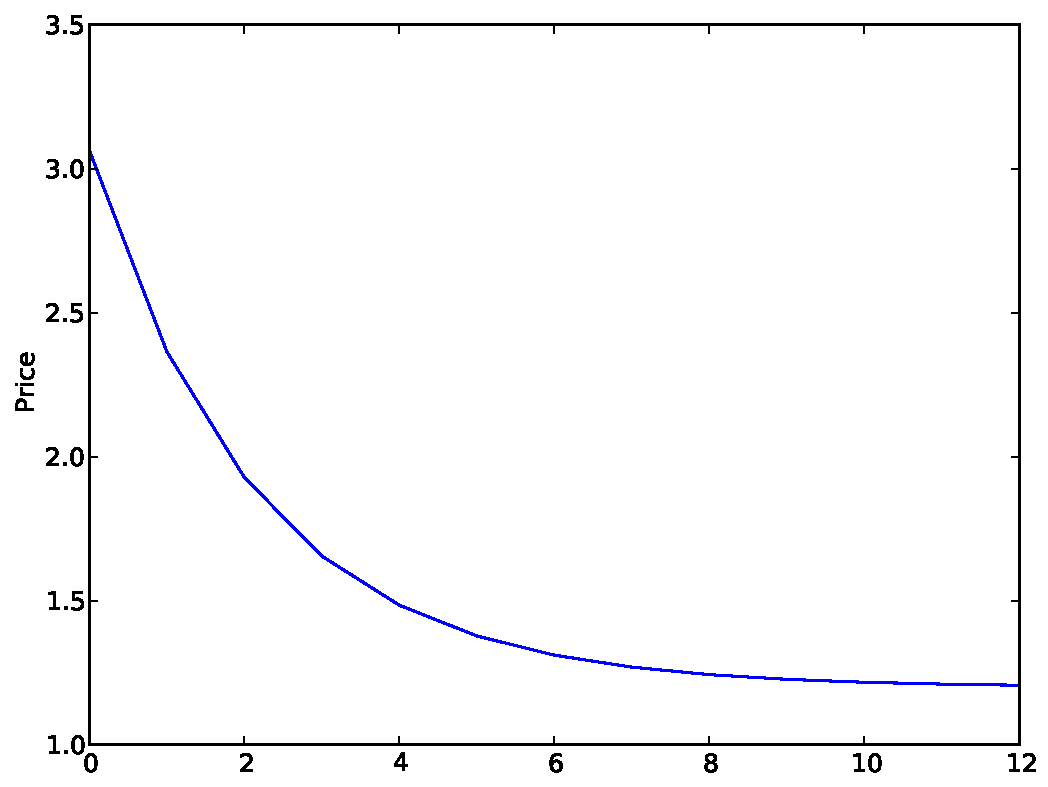
\includegraphics[scale=0.33]{conv_BC_price}
    \label{fig:conv_BC_price}
  } 
\subfloat[Regulator's tax]{
    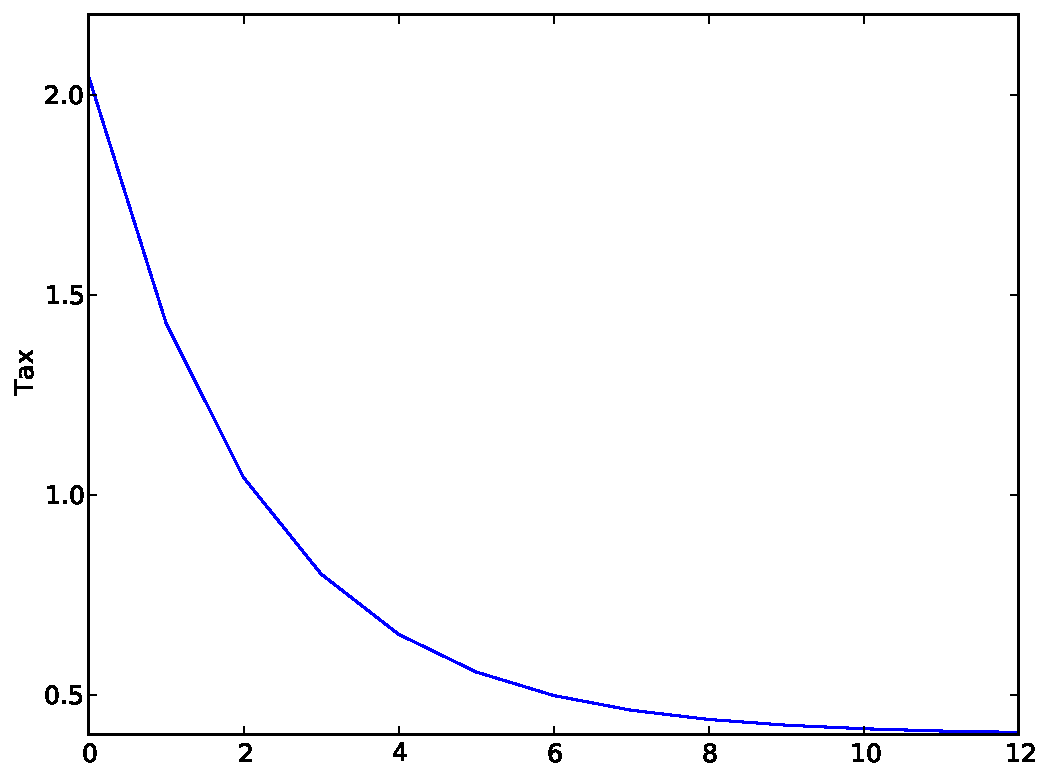
\includegraphics[scale=0.33]{conv_BC_tax}
    \label{fig:conv_BC_tax}
  }\newline
\subfloat[Demand]{
    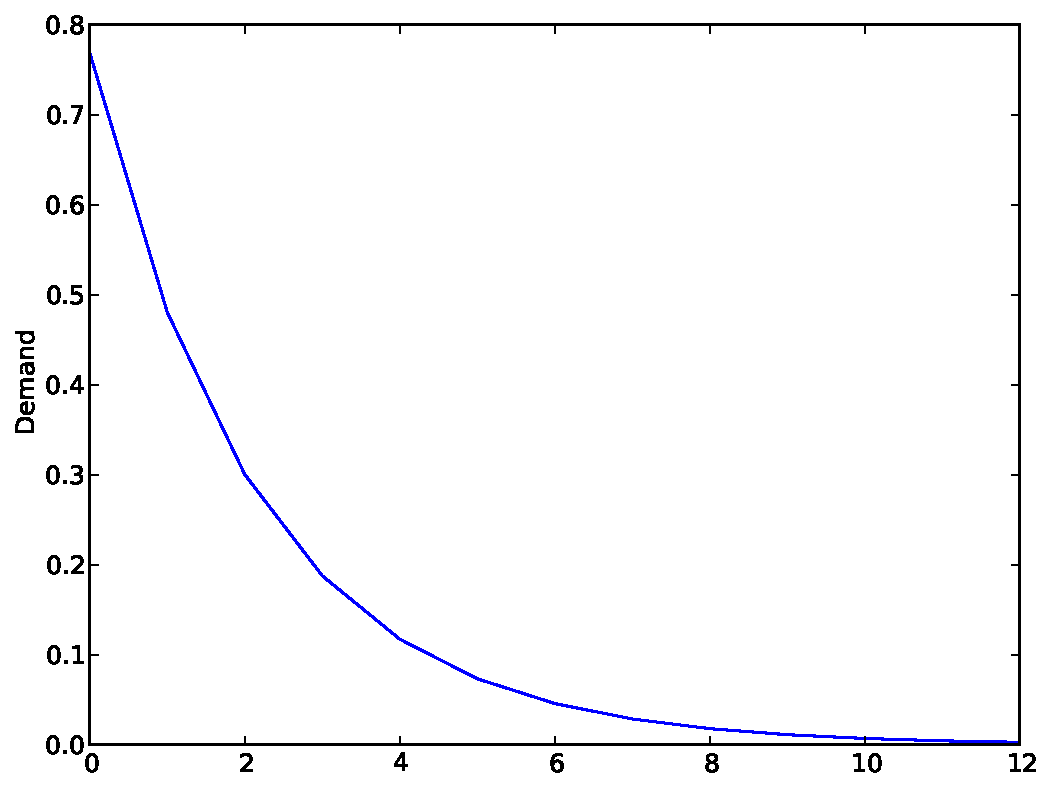
\includegraphics[scale=0.33]{conv_BC_demand}
    \label{fig:conv_BC_demand}
  } 
\subfloat[Monopolist's profit]{
    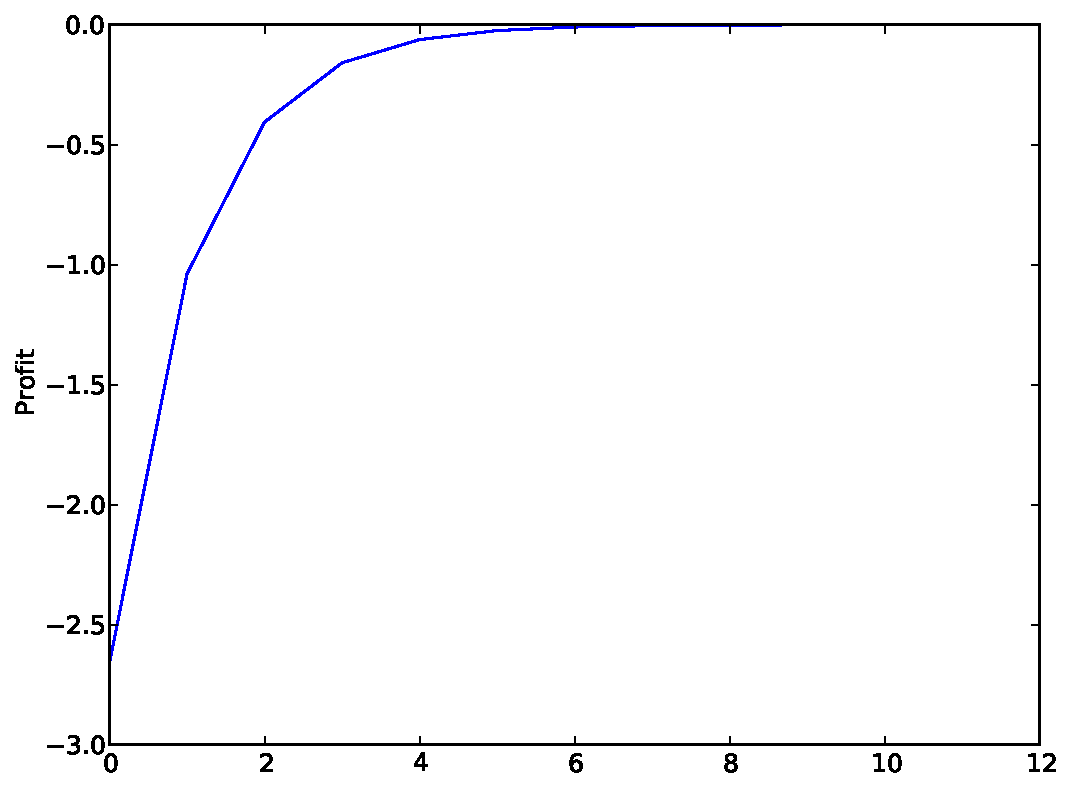
\includegraphics[scale=0.33]{conv_BC_profit}
    \label{fig:conv_BC_profit}
  }\newline
\subfloat[Pollution]{
    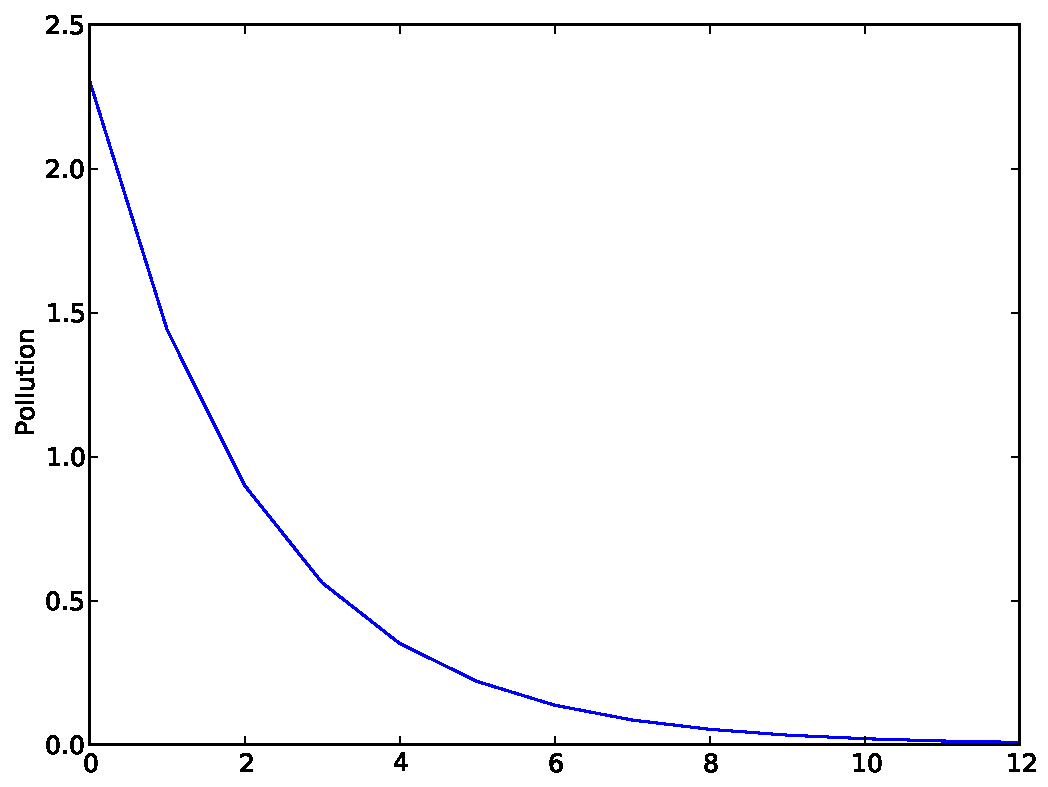
\includegraphics[scale=0.33]{conv_BC_pollution}
    \label{fig:conv_BC_pollution}
  } 
\subfloat[Welfare]{
    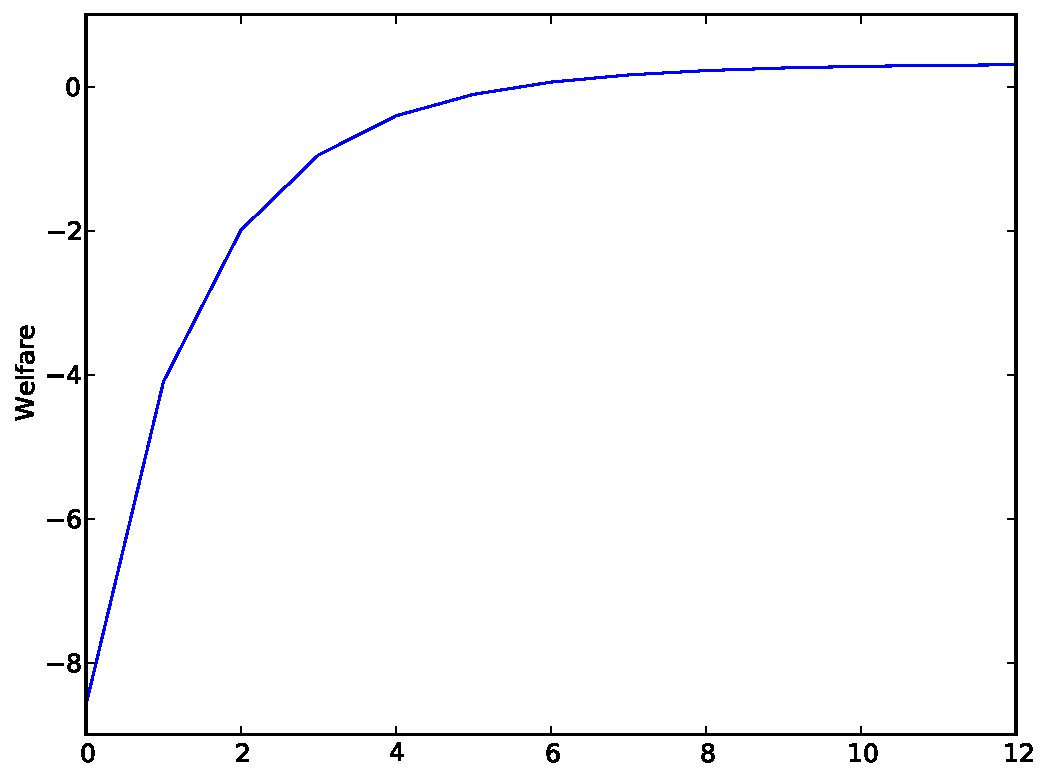
\includegraphics[scale=0.33]{conv_BC_welfare}
    \label{fig:conv_BC_welfare}
  }
\caption{Convergence in the base case over $12$ periods}
\label{fig:conv_BC_plots}
\end{figure}

The price is falling over time as the market participants with the greatest
valuation of the good purchase and exit the market. Therefore, condition %
\eqref{eq:1} is satisfied. The price gradually converges towards a steady
state of $\bar{p}\approx 1.2$ (see Appendix \ref{cha:numerical-results} for
a precise value). It should be noted that the steady state is an asymptote
of the price trajectory and is not reached in finite time.

Demand declines over time as the price differences across periods diminish.
If the price were to reach the steady state level, demand would drop to
zero. But since the steady state is approached only asymptotically, demand
is positive in all periods. As demand declines, so does the level of
pollution generated by production (Figure \ref{fig:conv_BC_pollution}).

Notably, firm profits are negative in this example. This raises the question
of why would this firm want to stay in business. Remember that the profits
reported in Figure \ref{fig:conv_BC_profit} are after-tax. Pre-tax profits
happen to be positive in all periods. As the monopolist cares about net
profits, the regulator could return the tax revenues to the monopolist as a
lump-sum transfer to keep him in business. Indeed, the point of taxation in
this model is to induce optimal behaviour, not to redistribute wealth. Thus,
there is nothing inherently objectionable about returning the revenues to
the monopolist. So long as the government's transfers to the monopolist are
not conditional on the current state variables, the efficiency of the
monopolist's decisions will not be affected.

Given our initial conditions, the equilibrium tax rate is also declining
over time as pollution levels are reduced. In the steady state the level of
taxation is about a third of the sale price ($\bar{\tau}\approx 0.4$). The
declining pollution externality reduces the need for taxation to alleviate
the problem. In addition, the monopolist's time inconsistency causes them to
charge a lower price in the current period in order to offset their
incentive for a price reduction in the following period. As prices in
consecutive periods converge over time, that incentive is reduced.
Consequently, the level of taxation required to correct for the monopolist's
inconsistency also declines.

The final variable charted in Figure \ref{fig:conv_BC_plots} is
instantaneous welfare. It is initially negative but converges to a positive
value as the pollution level drops. The positive value of the welfare is
driven by consumer surplus.

So far, the convergence paths of each variable in the base case accord with
what might be expected. Having canvassed them, we now turn to variations of
the parameters in Table \ref{tab:jmp_params} and the effect that such
variations have on the convergence paths and steady state levels of $\bar{p}$
and $\bar{\tau}$.

\section{Varying parameters}

\label{sec:varying-parameters-1}

Variation of the parameters is conducted in two parts. First, variations
that affect the convergence paths are considered. The simulation results
demonstrate that the parameters with the greatest impact upon convergence
paths are the time preference parameters, $\delta$ and $\beta$. The
remaining parameters have a negligible effect upon convergence rates: it
would not be visible at the scale plotted above in Figure \ref%
{fig:conv_BC_plots}. Consequently, convergence plots are given only for
those two variables.

The implications of the remaining variables for the equilibrium outcome are
analysed solely through their effect on the steady state levels $\bar{p}$
and $\bar{\tau}$.

\subsection{Convergence across parameter values}

\label{sec:conv-across-param}

In this subsection, the effect of varying the time preference parameters on
convergence rates is investigated.

\subsubsection{Varying $\protect\beta$}

\label{sec:varying-beta}

The first parameter that we vary is $\beta $, the consumer discount rate. It
embodies both the rate of consumer time preference and the depreciation rate
of the durable good. Consequently, it is rather lower than one might expect
for an ordinary time preference rate. In the base case, we set it to $\beta
=0.5$. For the variation we consider a range of values between $0.49$ and $%
0.52$. Beyond that range the steady state of the system is not in the
neighbourhood of the base case.

\begin{figure}[]
\centering
\subfloat[Monopolist's price]{
    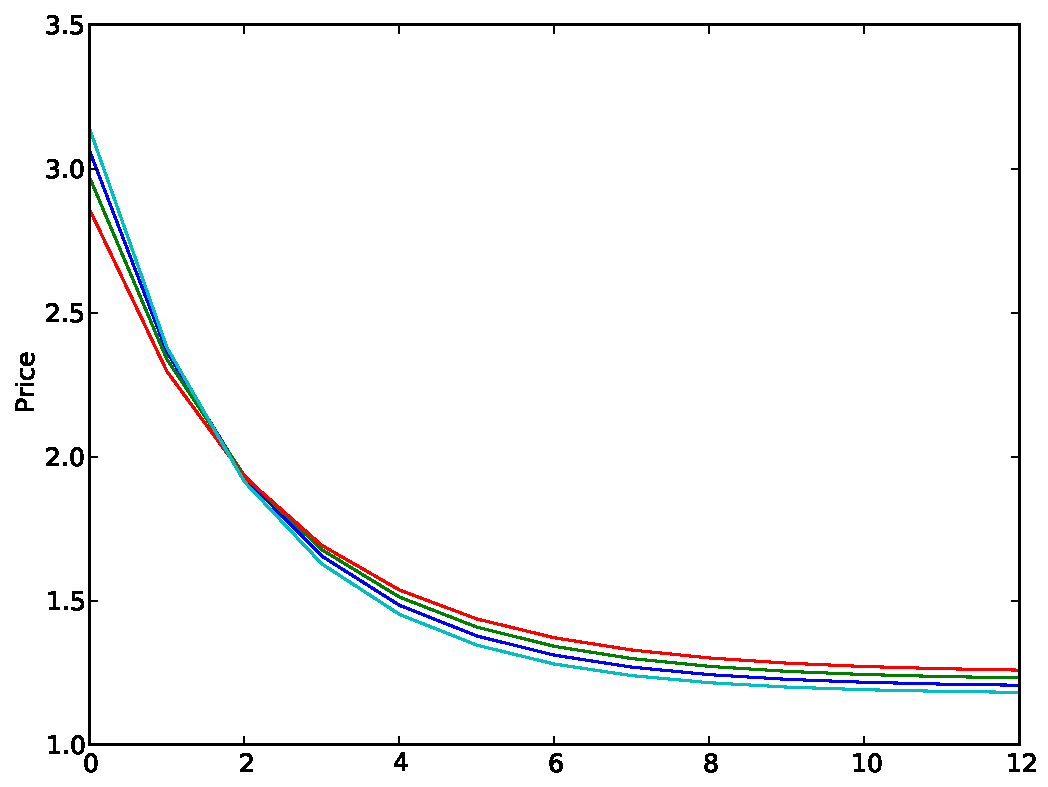
\includegraphics[scale=0.33]{conv_Beta_price}
    \label{fig:conv_Beta_price}
  } 
\subfloat[Regulator's tax]{
    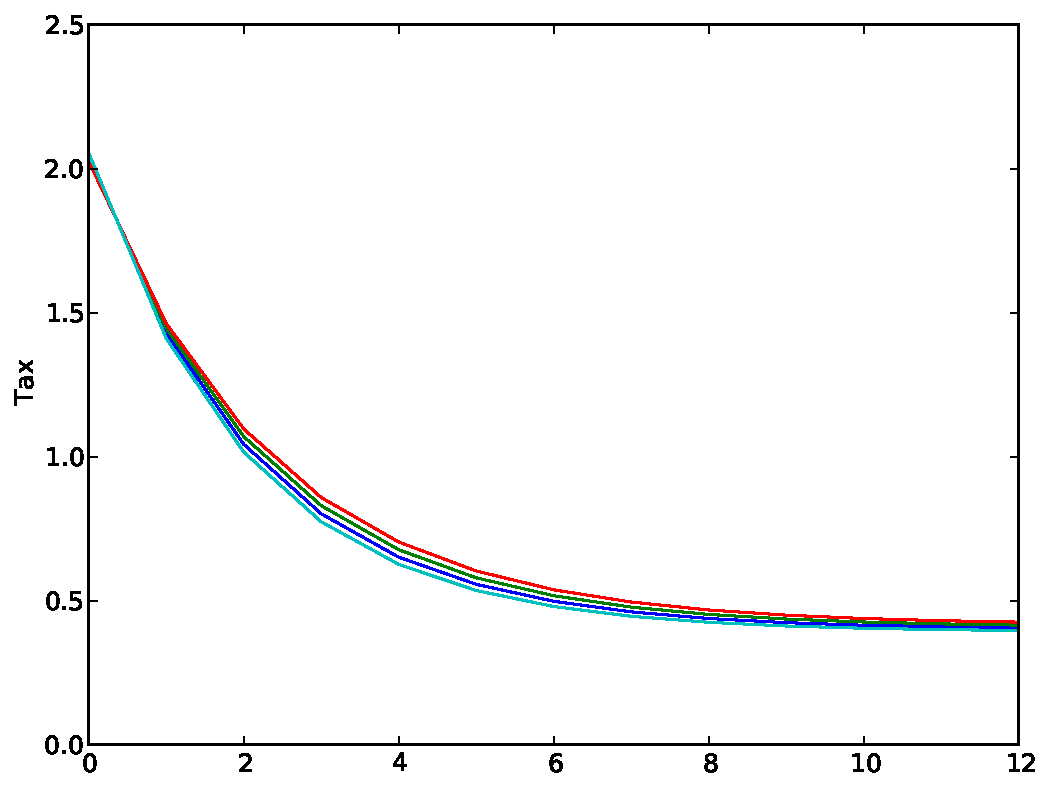
\includegraphics[scale=0.33]{conv_Beta_tax}
    \label{fig:conv_Beta_tax}
  }\newline
\subfloat[Demand]{
    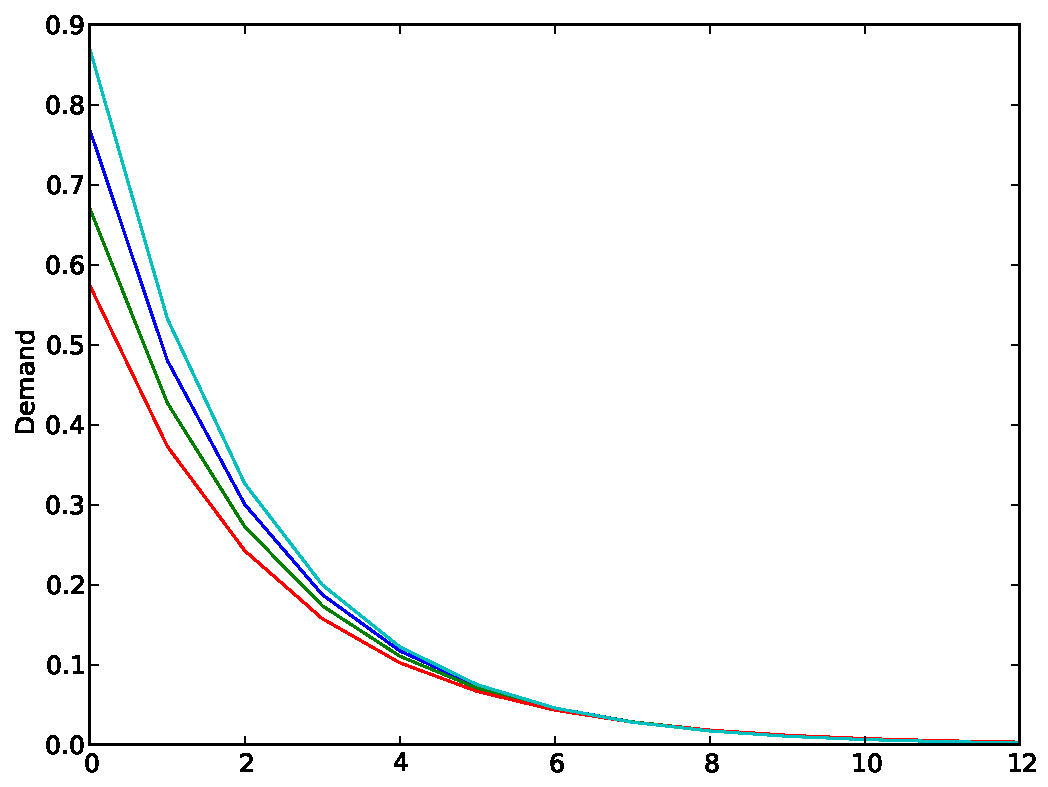
\includegraphics[scale=0.33]{conv_Beta_demand}
    \label{fig:conv_Beta_demand}
  } 
\subfloat[Monopolist's profit]{
    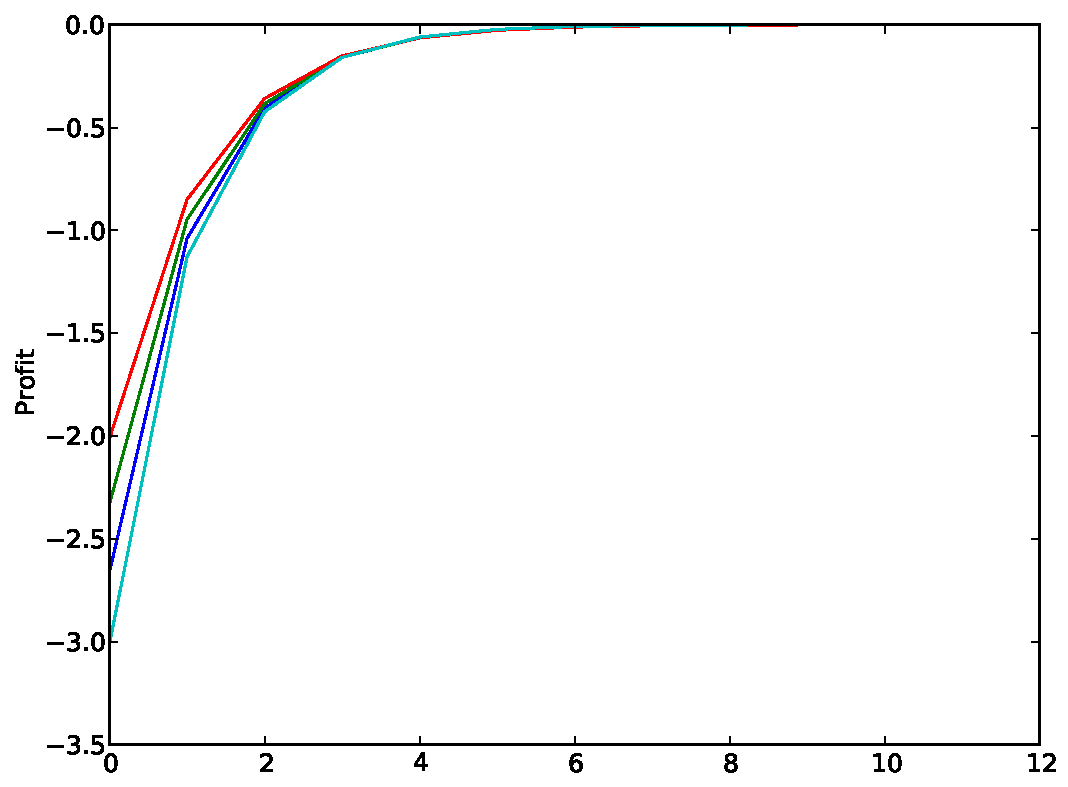
\includegraphics[scale=0.33]{conv_Beta_profit}
    \label{fig:conv_Beta_profit}
  }\newline
\subfloat[Pollution]{
    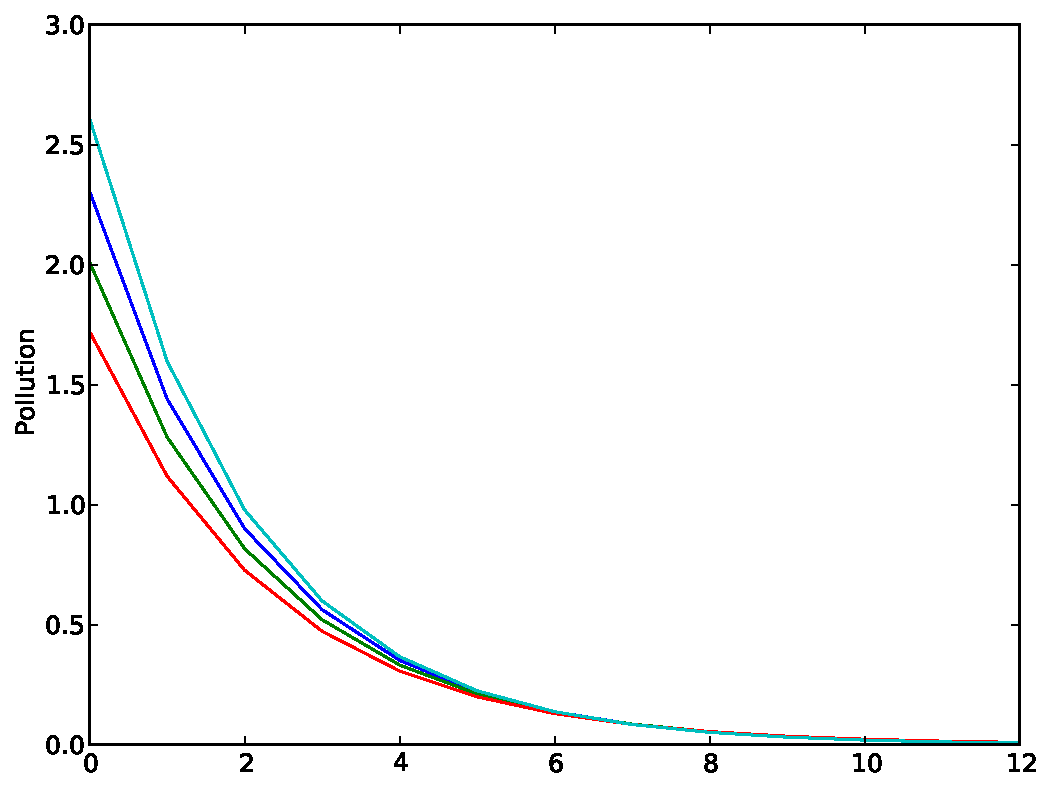
\includegraphics[scale=0.33]{conv_Beta_pollution}
    \label{fig:conv_Beta_pollution}
  } 
\subfloat[Welfare]{
    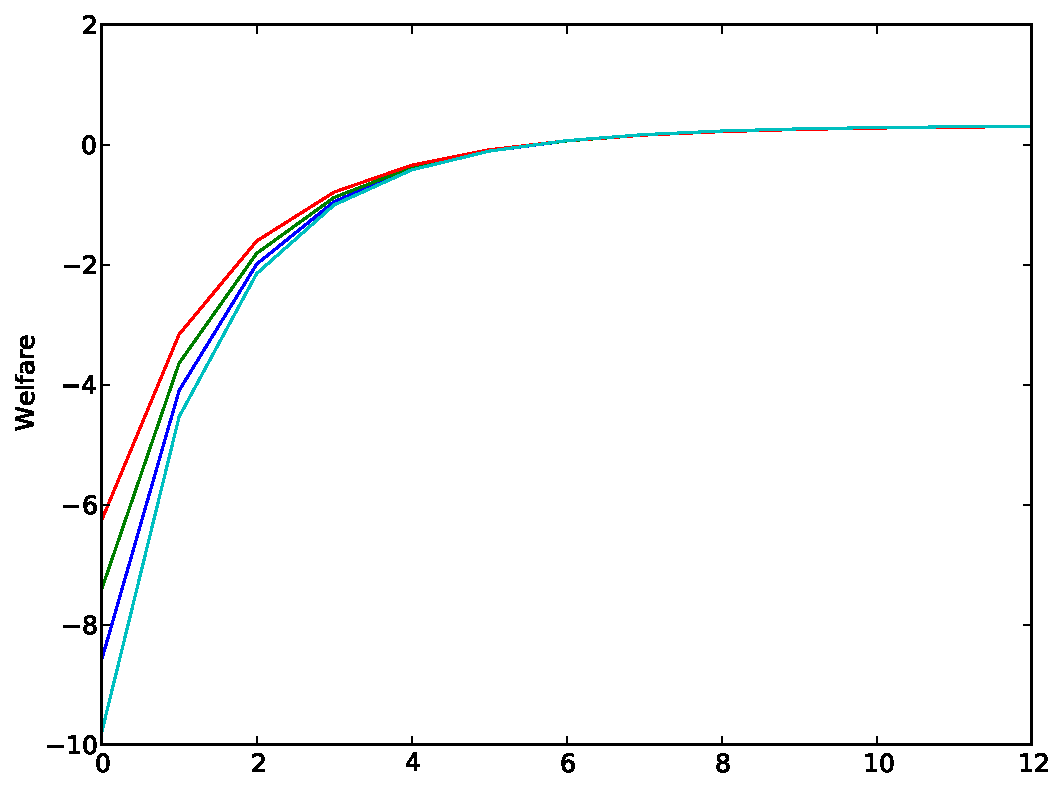
\includegraphics[scale=0.33]{conv_Beta_welfare}
    \label{fig:conv_Beta_welfare}
  }
\caption{Convergence for $\protect\beta \in \{0.49, 0.5, 0.51, 0.52\}$}
\label{fig:conv_beta_plots}
\end{figure}

The results are shown in Figure \ref{fig:conv_beta_plots} where $\beta =0.49$%
. The lower end of the range is denoted by the pale blue line and $\beta
=0.52$, at the upper end, is in red. The first thing to notice is that the
trajectory of demand is steeper when $\beta $ is lower. A lower value of $%
\beta $ decreases the value of postponing consumption, as the perceived
value of the durable good in the next period is lower. Consequently,
socially optimal consumption is shifted to earlier periods and demand is
initially higher but falls more quickly since there is a constant mass of
consumers. The increase in demand in early periods also pushes up pollution
levels and results in higher total pollution flows, which also cost the
monopolist profits due to the higher taxation. Interestingly, despite the
higher pollution levels the regulator chooses not to change the tax rate
significantly across the range of $\beta $'s tested.

\subsubsection{Varying $\protect\delta$}

\label{sec:varying-delta}

\begin{figure}[]
\centering
\subfloat[Monopolist's price]{
    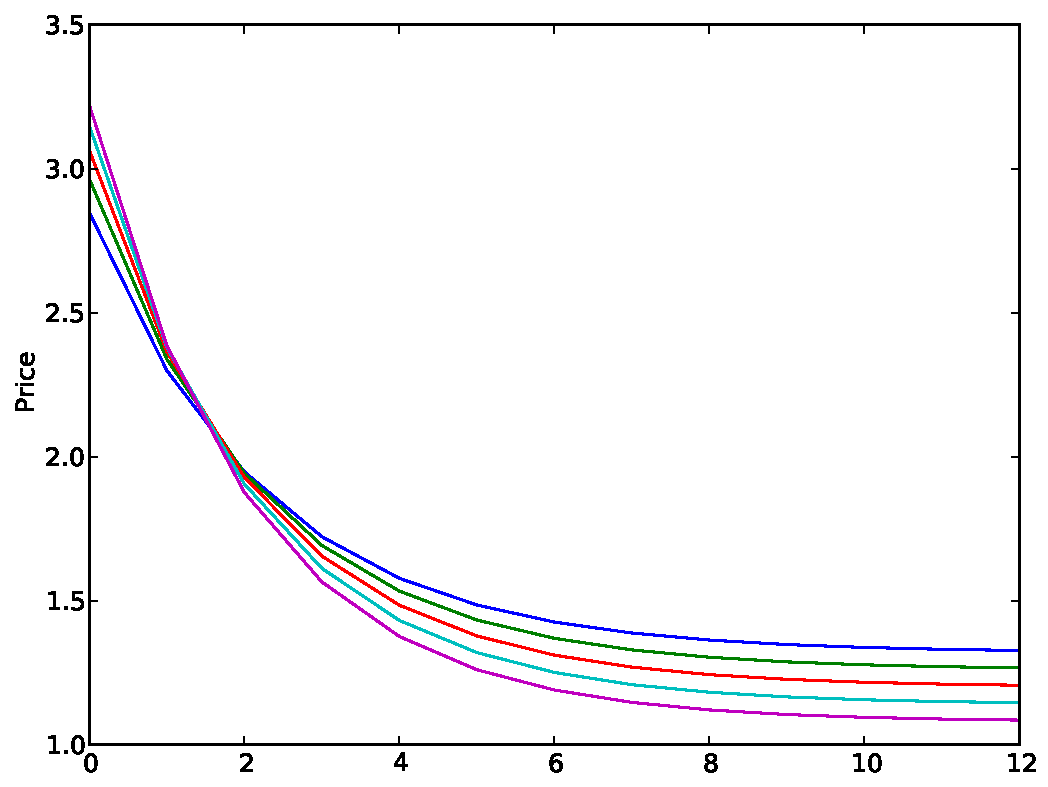
\includegraphics[scale=0.33]{conv_Delta_price}
    \label{fig:conv_Delta_price}
  } 
\subfloat[Regulator's tax]{
    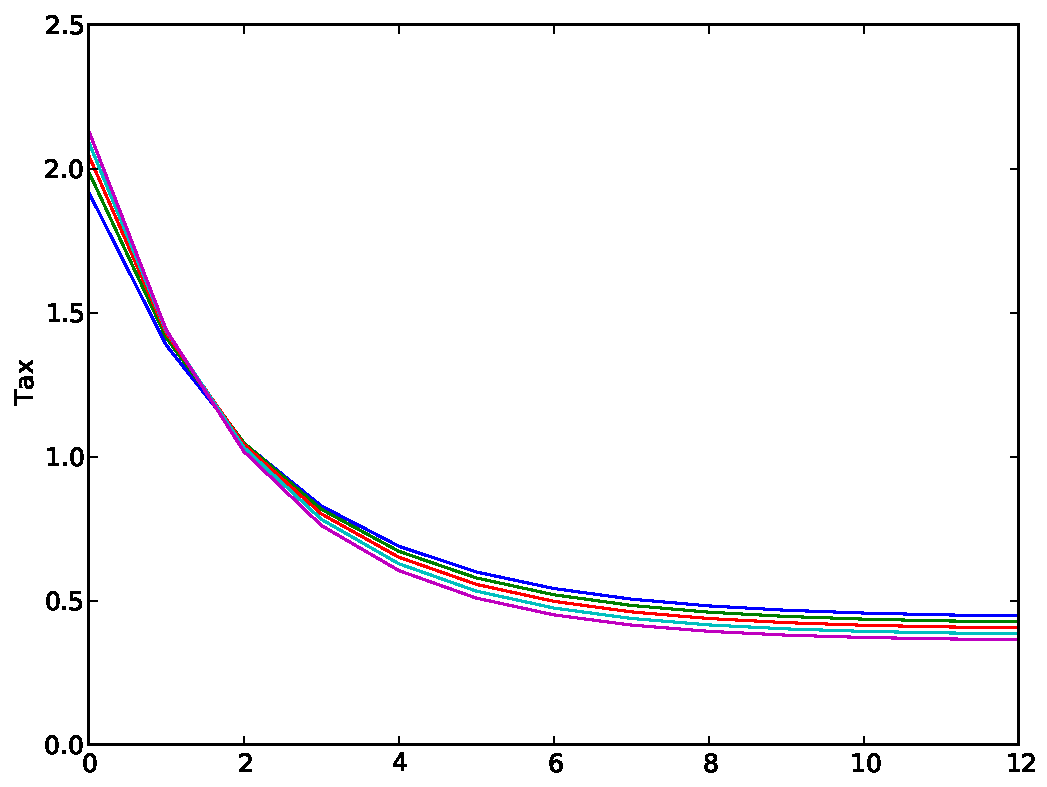
\includegraphics[scale=0.33]{conv_Delta_tax}
    \label{fig:conv_Delta_tax}
  }\newline
\subfloat[Demand]{
    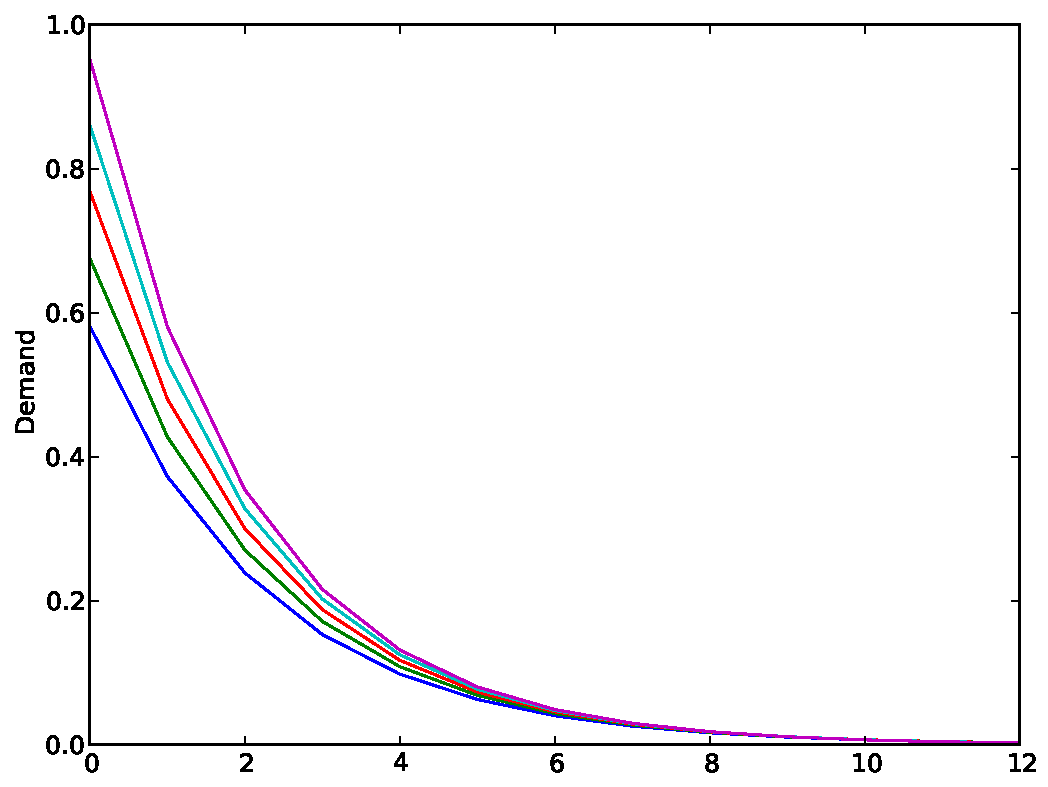
\includegraphics[scale=0.33]{conv_Delta_demand}
    \label{fig:conv_Delta_demand}
  } 
\subfloat[Monopolist's profit]{
    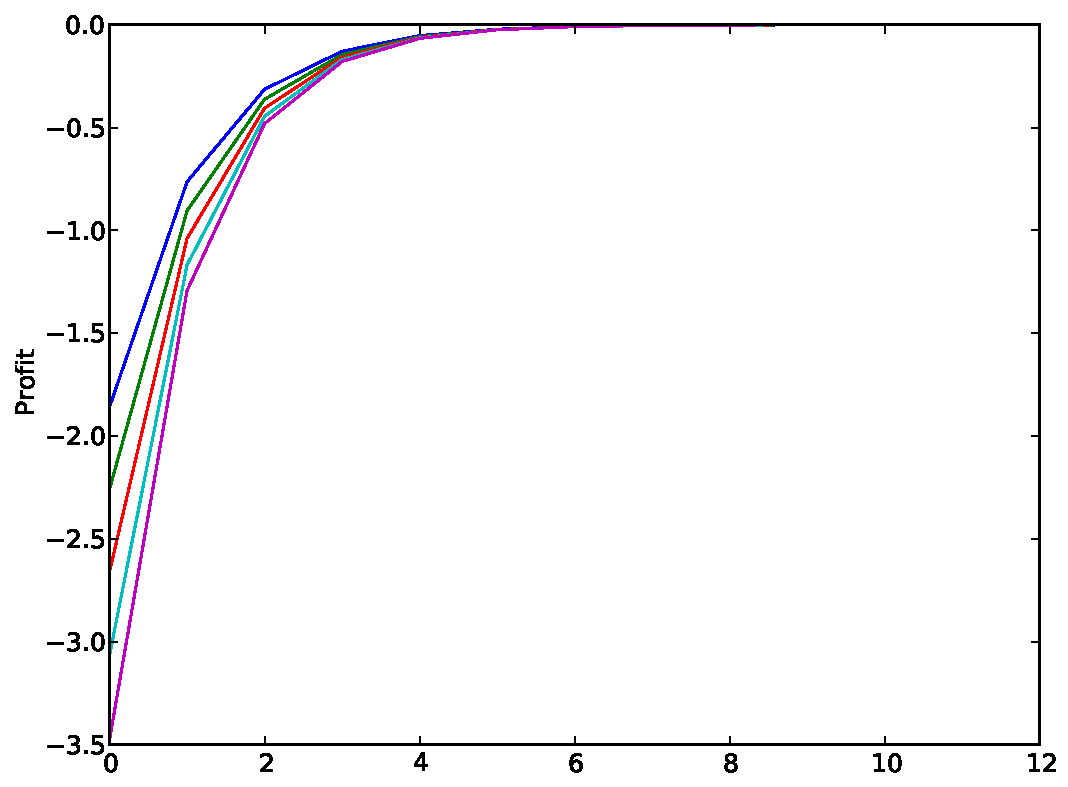
\includegraphics[scale=0.33]{conv_Delta_profit}
    \label{fig:conv_Delta_profit}
  }\newline
\subfloat[Pollution]{
    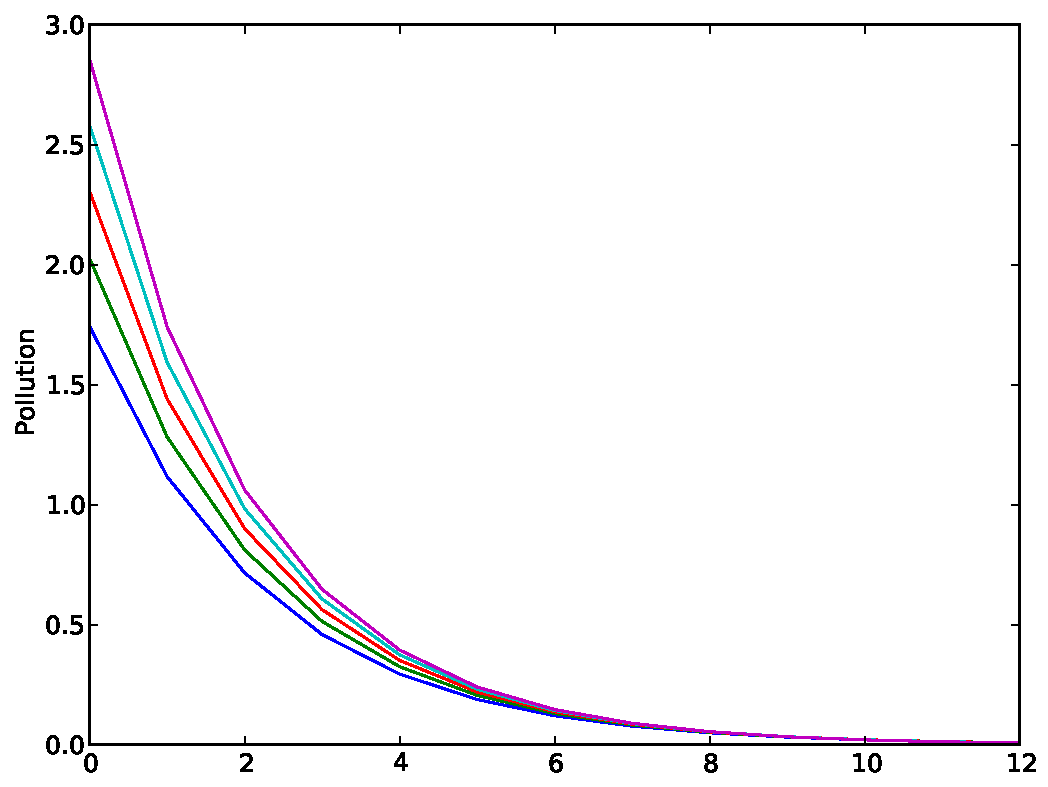
\includegraphics[scale=0.33]{conv_Delta_pollution}
    \label{fig:conv_Delta_pollution}
  } 
\subfloat[Welfare]{
    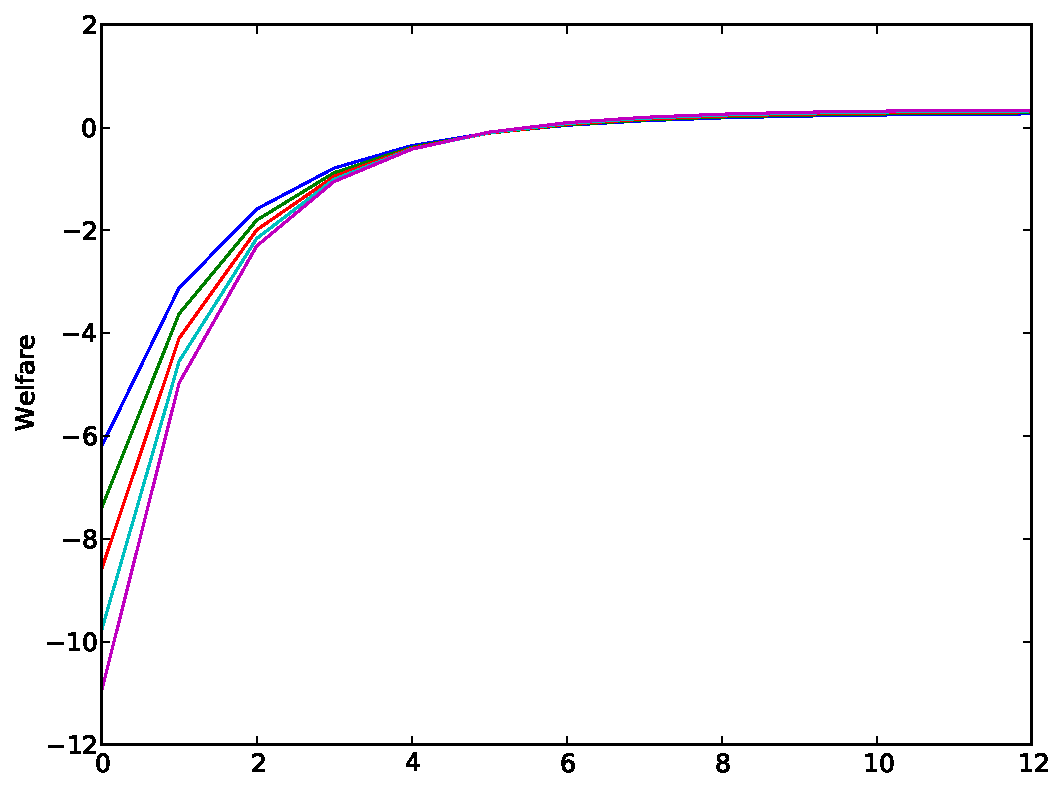
\includegraphics[scale=0.33]{conv_Delta_welfare}
    \label{fig:conv_Delta_welfare}
  }
\caption{Convergence for $\protect\delta \in \{0.78, 0.79, 0.8, 0.81, 0.82\}$
}
\label{fig:conv_delta_plots}
\end{figure}

The final part of our examination of convergence is an investigation of
variations of the discount factor of the government and the monopolist, $%
\delta $. It describes how future payoffs are valued relative to the current
period's payoff in the taxation game. The results are shown in Figure \ref%
{fig:conv_delta_plots} and are very similar to the results for variation in $%
\beta $, as one might expect for another time preference parameter.

The only notable differences are in the magnitude of the effect and the
impact upon the tax rate. The magnitude of the effect is slightly greater
since $\beta$ influences all future values, rather then solely consumers'
valuations of the durable good. However, it is the path of the tax rate that
is more interesting.

In Figure \ref{fig:conv_Beta_tax} the tax rate varied little between
different values of $\beta$ whereas, in Figure \ref{fig:conv_Delta_tax}, the
tax rate shows similar variation to the price path.

\subsection{Steady states across parameter values}

\label{sec:steady-states-across}

\begin{figure}[ht]
\centering
\subfloat[$\beta \in \{ 0.49, 0.5, 0.51, 0.52 \}$, $\delta \in \{
   0.78, 0.79, 0.8, 0.81, 0.82 \}$]{
    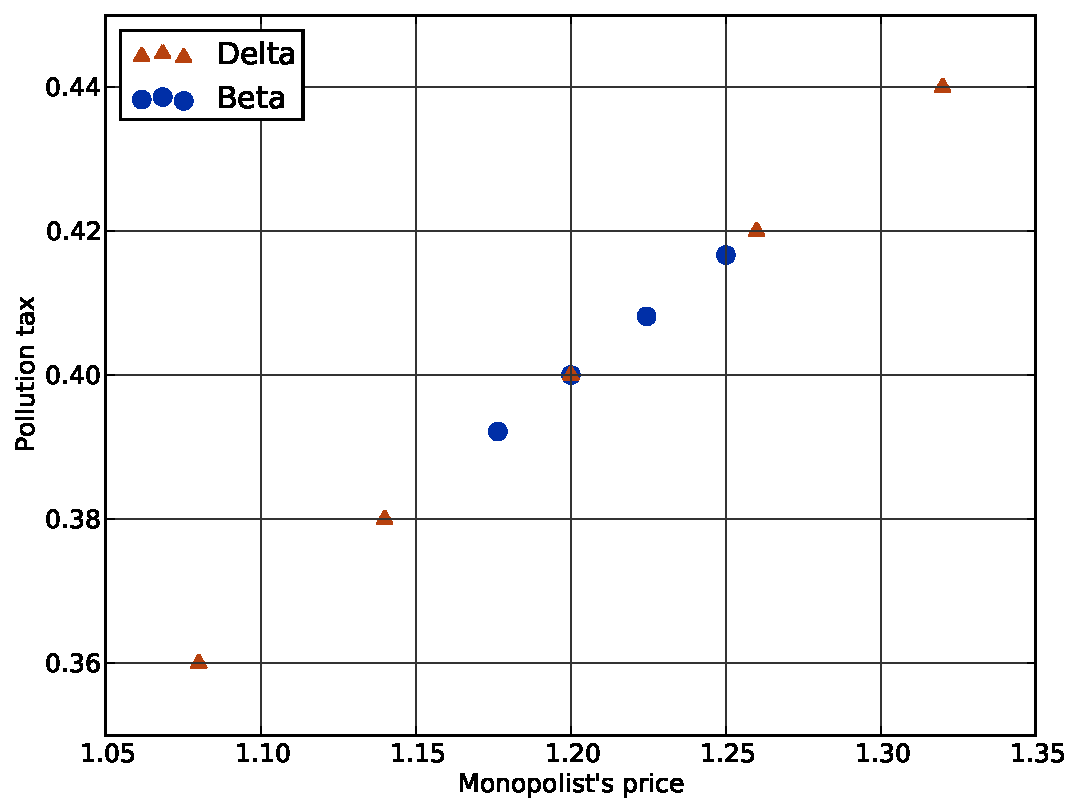
\includegraphics[scale=0.4]{SS_beta_delta}
    \label{fig:SS_beta_delta}
  }\newline
\subfloat[$\kappa \in \{ 2.98, 2.99, 3, 3.01, 3.02 \}$, $\alpha \in
   \{ 0.98, 0.99, 1 \}$]{
    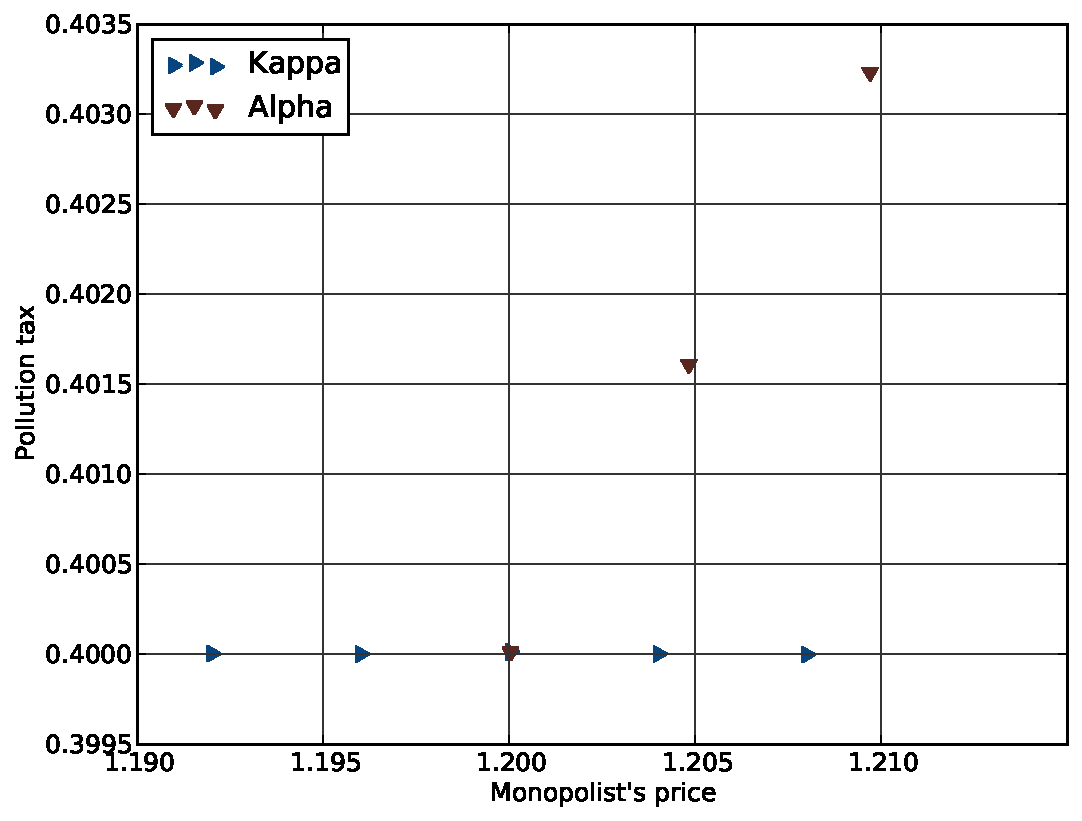
\includegraphics[scale=0.4]{SS_kappa_alpha}
    \label{fig:SS_kappa_alpha}
  }\newline
\subfloat[$\theta \in \{ 0, 0.01, 0.02 \}$, $\rho \in \{ 0.98,
   0.99, 1, 1.01, 1.02 \}$]{
    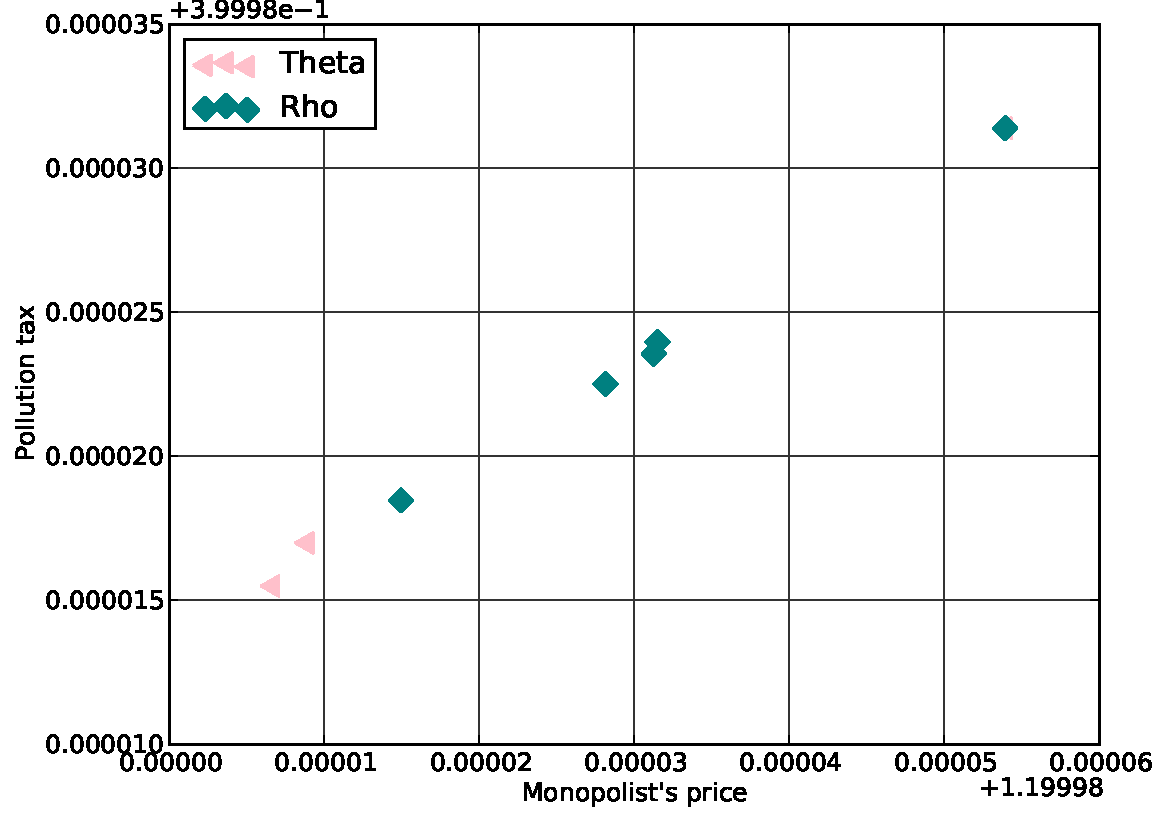
\includegraphics[scale=0.4]{SS_theta_rho}
    \label{fig:SS_theta_rho}
   }
\caption{Variation in steady states across parameter values}
\label{fig:ss_plots}
\end{figure}

Having examined the impact on convergence of time preference rates we now
turn to the steady state comparison. In this subsection we focus on the
difference in steady states as the parameters vary. Figure \ref{fig:ss_plots}
shows a scatter plot of $\bar{p}$ and $\bar{\tau}$ for pairs of parameter
values. The pairs are chosen by the magnitude of their effect so the scale
of the plot shrinks from Figure \ref{fig:SS_beta_delta} through to Figure %
\ref{fig:SS_theta_rho}.

A indicated in the previous section, the time preference rates have the
greatest impact on the result and in a similar fashion; $\delta$ with
greater magnitude than $\beta$. That is clearly shown by Figure \ref%
{fig:SS_beta_delta}, which indicates that the effect of each on the steady
state is identical in direction and varies only in magnitude. As agents
reduce their valuation of future payoffs the monopolist is forced to lift
their production and reduce their price in order to maintain demand for
their product. That, in turn generates pollution and causes a commensurate
lift in the tax rate to compensate.

In Figure \ref{fig:SS_kappa_alpha} the government's valuation of tax
revenues, $\alpha$, and the pollution function's coefficient, $\kappa$, are
varied. The effect of a drop in $\alpha$ is to increase the tax rate levied
by the regulator while changing the rate of pollution has no effect upon the
tax rate but does affect the price charged by the monopolist.

Finally, Figure \ref{fig:SS_theta_rho} shows the negligible impact that the
cost of policy changes, $\theta$, and the production cost coefficient, $\rho$%
, have on the steady state. Increasing $\rho$ causes the monopolist to
increase prices, as might be expected when their marginal costs rise;
however, the scale of the impact is such that it is an insignificant effect
relative to that of time preference and the coefficient on pollution.

%%% Local Variables:
%%% mode: latex
%%% TeX-master: "root"
%%% End:


\chapter[Hyperbolic discounting]{Extension: a quasi-hyperbolic discounting
model}

\label{cha:model}

In Chapter \ref{sec:dynamic-consistency} we mentioned that there are two
main causes of dynamic inconsistency: jump states and hyperbolic
discounting. The prior chapters of this thesis have dealt extensively with
the issue of regulation in the presence of jump states. We developed a
variant of a strategic delegation game to deal with inconsistency implied by
a jump state. Inefficiencies due to hyperbolic discounting can be addressed
in a similar way. In this chapter we demonstrate how the same mechanism can
also be used by a regulator who suffers from inconsistency due to
quasi-hyperbolic discounting.

We will argue that this type of inconsistency is different from the problem
posed by jump states. However, the taxation mechanism described in chapter %
\ref{cha:proposition} can still attain the socially optimal outcome.

\section{Quasi-hyperbolic discounting}

\label{sec:quasi-hyperb-disc}

Hyperbolic discounting models originated from \citet{Ainslie1992}'s
empirical work. He showed that a hyperbolic curve is a far better match for
the discount rate of most people than the standard exponential curve. When
agents use hyperbolic discounting, their intertemporal trade-offs are not
time invariant. Thus, such discount functions are not as mathematically easy
to work with as exponential functions. Because of this difficulty Ainslie's
book did not get the attention it deserved until the modifications by %
\citet{Laibson1997} which made the analysis more tractable.

Rather than adopting a full hyperbolic function, Laibson introduced an
exponential function with a modifier on the current period's discount rate.
In Laibson's model, the discount factor for the next period is $\beta \delta 
$, where $0<\beta <1$ and $0<\delta <1$. All subsequent periods are
discounted exponentially by a factor $\delta $. This modification makes the
model both simple to work with and a fair approximation of a hyperbolic
function. Time preferences with this structure are known as quasi-hyperbolic
preferences.

Quasi-hyperbolic discounting captures non-stationary time preferences, \`{a}
la hyperbolic discounting, while preserving analytical tractability.
Non-stationarity gives rise to time inconsistency, as the intertemporal
trade-off between two successive periods will change with the agent's time
reference. Consequently, precommitment has value similar to that in models
with jump states.

In the following two chapters we develop a simple quasi-hyperbolic
discounting model analogous to the monopolistic model of Chapter \ref%
{cha:problem}. Then we demonstrate the ability of the taxation game to
correct both the regulator's time inconsistency as well as the pollution
externality.

\section{The quasi-hyperbolic model}

\label{sec:quasi-hyperb-model}

As before, this model also involves a monopolist producing a good that
creates a pollution externality. The regulator addresses inefficiencies
caused by this externality through Pigouvian taxation. However, the
regulator suffers from self-control problems induced by quasi-hyperbolic
time preferences.

\section{Elements of the model}

\label{sec:elements-model}

The description of our model begins with a characterisation of the agents: a
consumer, a monopolist and a regulator.

\subsection{The consumer}

\label{sec:consumer}

Imagine a representative consumer who derives utility from two goods: a
polluting good, $x$, and a numeraire, $m$. The consumer's instantaneous
utility function is 
\begin{equation}
U(x,m)=u(x)+m.  \label{eq:27}
\end{equation}%
We assume that $u(x)$ satisfies the Inada conditions. This ensures that the
inverse demand is well-defined for all positive values of $x$.

The consumer's budget constraint is 
\begin{equation}
px+m=I.  \label{eq:28}
\end{equation}%
Therefore, inverse demand in this market is given by 
\begin{equation}
p=u^{\prime }(x).  \label{eq:31}
\end{equation}

\subsection{The monopolist}

\label{sec:monopolist}

The market for good $x$ is served by a monopolist with a cost function $C(x)$%
. His instantaneous profit function is 
\begin{align}
\pi (x)& =R(x)-C(x)  \label{eq:32} \\
& =px-C(x).
\end{align}%
Equation \eqref{eq:31} implies that profit can also be written as 
\begin{equation}
\pi (x)=u^{\prime }(x)x-C(x).  \label{eq:81}
\end{equation}

The monopolist has standard exponential time preferences and is thus time
consistent.

\subsection{The regulator}

\label{sec:regulator}

Production generates a pollution externality that is not internalised by the
monopolist. Unlike in the previous chapters, here pollution is modelled as a
stock externality rather than a flow externality. The regulator has
oversight of the monopolist and seeks to mitigate the damage wrought by the
monopolist's emissions. The stock of pollution generated by the production
of good $x$ at time $t$ is denoted by $k_{t}$.\footnote{%
For tractability in this model we have switched from flow pollution to stock
pollution.} The environmental harm caused by this stock is $\phi (k_{t})$,
where $\phi ^{\prime }(k_{t})>0$.

The stock of pollution evolves according to the following law-of-motion: 
\begin{equation}
k_{t}=\theta k^{t-1}+x^{t-1}.  \label{eq:33}
\end{equation}%
The parameter $\theta \in \lbrack 0,1]$ represents the rate of pollution
carry-over. Instantaneous welfare is thus given by 
\begin{align}
w(x_{t},k_{t})& =\pi (x_{t})+CS(x_{t})-\phi (k_{t})  \label{eq:83} \\
& =u^{\prime }(x_{t})x_{t}-C(x_{t})+\int_{0}^{x_{t}}u^{\prime
}(x)\;dx-u^{\prime }(x_{t})x_{t}-\phi (k_{t}) \\
& =u(x_{t})-C(x_{t})-\phi (k_{t}).
\end{align}

The regulator suffers from time inconsistency and is modelled as having
quasi-hyperbolic preferences. In particular, his net present valuation of
welfare from the period-$t$ perspective is 
\begin{equation}
W_{t}=w(x_{t},k_{t})+\beta \sum_{i=1}^{\infty }\delta ^{i}w(x_{t+i},k_{t+i}).
\label{eq:35}
\end{equation}%
Note the $\beta $ modifier in lifetime welfare. If $\beta =1$ then the
preferences are `exponential' and time consistent. If $\beta <1$, as is
assumed here, then preferences are `present biased' (i.e.\ non-stationary)
and the regulator will experience dynamic inconsistency.

\section{Laissez-faire equilibrium}

\label{sec:laiss-faire-equil}

First we consider the laissez-faire case. Suppose that the firm is not
regulated by the government. The monopolist does not account for the damages
arising from his pollution. As a result, the pollution stock does not appear
in his payoff. In each period, the firm solves the following static problem: 
\begin{equation}
\max_{x}u^{\prime }(x)x-C(x).  \label{eq:36}
\end{equation}

The first order condition of this problem is 
\begin{equation}
u^{\prime \prime }(x^{\ell })x^{\ell }+u^{\prime }\left( x^{\ell }\right)
-C^{\prime }\left( x^{\ell }\right) =0\text{,}  \label{eq:37}
\end{equation}%
where $x^{\ell }$ denotes the laissez-faire level of output chosen by the
monopolist. Intuitively, condition \eqref{eq:37} delivers the output level
at which marginal profit is equal to zero.

Since the monopolist discounts future payoffs exponentially, his lifetime
profit is 
\begin{equation}
\sum_{t=0}^{\infty }\delta ^{t}\pi _{t}=\frac{u^{\prime }\left( x^{\ell
}\right) x^{\ell }-C\left( x^{\ell }\right) }{1-\delta }\text{.}
\label{eq:82}
\end{equation}

\section{Benchmarking regulation}

\label{sec:benchm-regul}

\subsection{First best regulation}

\label{sec:first-best-regul}

Before we analyse the taxation game, let us first benchmark the performance
of a regulator who could choose output levels. Again, we first examine the
problem of a hypothetical regulator who can both directly determine output
and perfectly precommit to future policies. 

Suppose that the regulator can directly choose the lifetime output plan $%
\{x_{t}\}_{t=0}^{\infty }$ at time $0$. The optimal plan would solve 
\begin{multline}
W_{0}=u(x_{0})-C(x_{0})-\phi (k_{0})  \label{eq:38} \\
+\beta \sum_{t=1}^{\infty }\delta ^{t}\left[ u(x_{t})-C(x_{t})-\phi (k_{t})%
\right]
\end{multline}%
where the state variable evolves according to%
\[
k_{t}=\theta k_{t-1}+x_{t-1}, 
\]%
$\delta $ is the discount rate and $\beta $ is the quasi-hyperbolic modifier
on the future discount factor.

The regulator's optimal choice will satisfy 
\begin{equation}
w_{1}^{0}+\beta \delta \left( w_{2}^{1}-\theta w_{1}^{1}\right) =0
\label{eq:86}
\end{equation}%
in period 0, and 
\begin{equation}
w_{1}^{t}+\delta \left( w_{2}^{t}-\theta w_{1}^{t+1}\right) =0\qquad \forall
\;t\geq 2.  \label{eq:87}
\end{equation}%
for each subsequent period $t$. See Appendix \ref{sec:first-best-regul-1}
for more detail. \ 

Equations \eqref{eq:86} and \eqref{eq:87} together characterise the output
path the regulator would choose, were he able to directly control output
levels. From the perspective of the regulator at time $0$, this is the first
best output path. After substituting $w(x_{t},k_{t})$ from \eqref{eq:83}, we
obtain%
\begin{equation}
u^{\prime }(x_{t})-C^{\prime }(x_{t})-\delta \theta \left( u^{\prime
}(x_{t+1})-C^{\prime }(x_{t+1})\right) -\delta \phi ^{\prime
}(k_{t+1})=0\qquad \forall \;t\geq 2.  \label{eq:45}
\end{equation}%
This equation will be used for comparison with the laissez-faire condition,
as they have similar forms.

\subsection{Comparison to laissez-faire outcome}

\label{sec:comp-laiss-faire}

It is instructive to compare the first-best outcome to the laissez-faire
equilibrium characterised in equation \eqref{eq:37}: 
\begin{equation}
u^{\prime }\left( x^{\ell }\right) -C^{\prime }\left( x^{\ell }\right)
+u^{\prime \prime }\left( x^{\ell }\right) x^{\ell }=0.  \label{eq:46}
\end{equation}%
Remember that this condition sets the monopolist's marginal profit to zero.
Since profit is concave, marginal profit is a decreasing function.

We focus on the steady state of the model. Suppose that $x_{t}=\bar{x}%
,\forall t$, and thus $k_{t}=\bar{k},\forall t$. Now rearrange equation %
\eqref{eq:45}, 
\begin{equation}
u^{\prime }\left( \bar{x}\right) -C^{\prime }\left( \bar{x}\right) =\frac{%
\delta \phi ^{\prime }\left( \bar{k}\right) }{1-\delta \theta },
\label{eq:47}
\end{equation}%
and add $u^{\prime \prime }\left( \bar{x}\right) \bar{x}$ to both sides: 
\begin{equation}
u^{\prime }\left( \bar{x}\right) -C^{\prime }\left( \bar{x}\right)
+u^{\prime \prime }\left( \bar{x}\right) \bar{x}=\frac{\delta \phi ^{\prime
}\left( \bar{k}\right) }{1-\delta \theta }+u^{\prime \prime }\left( \bar{x}%
\right) \bar{x}.  \label{eq:48}
\end{equation}%
The left-hand side of the above equation represents the monopolist's
marginal profit evaluated at the steady-state first best output level.
Remember that marginal profit is a decreasing function. Thus, if $\frac{%
\delta \phi ^{\prime }\left( \bar{k}\right) }{1-\delta \theta }+u^{\prime
\prime }\left( \bar{x}\right) \bar{x}>0$ then $\bar{x}<x^{\ell }$ and vice
versa.

Signing the component parts gives 
\begin{align}
\delta \phi ^{\prime }\left( \bar{x}\right) & >0  \label{eq:49} \\
1-\beta \delta & >0 \\
u^{\prime \prime }\left( \bar{x}\right) \bar{x}& <0
\end{align}%
So if 
\begin{equation}
\frac{\delta \phi ^{\prime }\left( \bar{k}\right) }{1-\delta \theta }%
>u^{\prime \prime }\left( \bar{x}\right) \bar{x}  \label{eq:50}
\end{equation}%
then $\bar{x}<x^{\ell }$. The left hand side of the inequality represents
the lifetime marginal cost of the externality, while the right hand side is
the deadweight loss due to monopoly power. The externality implies that the
quantity produced may be too high from a welfare point of view, while the
firm's market power suggests that production could be too low. Taxing the
firm to reduce pollution is only worthwhile when the former effect outweighs
the latter. Henceforth, we shall assume that equation \eqref{eq:50} holds.

\subsection{Second best regulation}

\label{sec:second-best-regul}

Sophisticated regulators would recognise that they have a time inconsistency
problem. Therefore, they will try to avail themselves of a solution. If they
unable to precommit to future policies, they will act strategically to
influence the decisions of their future selves. Such behaviour would give
rise to a time-consistent second best-output path. This path would occur if
the regulator could directly choose output, but had no means of
precommitting themselves to future decisions.

To solve for the time consistent equilibrium, we must formulate the problem
recursively. Let the MPE strategy of the regulator be $x_{t}=f(k_{t})$. Then
his Bellman equation is 
\begin{equation}
U(k_{t})=\max_{x_{t}}\left\{ w(x_{t},k_{t})+\beta \delta V(\theta
k_{t}+x_{t})\right\}   \label{eq:51}
\end{equation}%
where $U(\cdot )$ is his current period's value function and $V(\cdot )$ is
his continuation value function. The continuation value function captures
the stream of future payoffs from period $t+1$ onward. It is different from
the current period's value function because quasi-hyperbolic preferences are
non-stationary. Since from next period onwards the regulator would discount
welfare exponentially, the continuation value function must satisfy the
recursive equation 
\begin{equation}
V(k_{t})=w\left( f(k_{t}),k_{t}\right) +\delta V\left( \theta
k_{t}+f(k_{t})\right) .  \label{eq:52}
\end{equation}

Dynamic programming renders a generalised Euler equation that characterises
the regulator's output strategy: 
\begin{equation}
w_{1}^{t}+\beta \delta (w_{1}^{t+1}f_{1}^{t+1}+w_{2}^{t+1})-\delta (\theta
+f_{1}^{t+1})w_{1}^{t+1}=0.  \label{eq:55}
\end{equation}

Note the difference between equation \eqref{eq:55} and equation \eqref{eq:87}%
. This difference suggests that the time consistent path will not coincide
with the first-best (i.e. precommitment) path.

\section{Regulation with delegation}

\label{sec:regul-with-deleg}

Intuitively it should be possible to solve a quasi-hyperbolic discounting
problem through `delegation' of the pricing decision.

Quasi-hyperbolic time preferences give rise to time inconsistent behaviour.
However, the internal strategic conflict between two successive regulators,
in periods $t$ and $t+1$, only concerns the choice of the period-$t+1$
action. These two regulators do not disagree about future actions, as both
will discount future payoffs exponentially. Thus, by eliminating the direct
effect of today's decision on next period's payoff, it should be possible to
render the regulator consistent.

In our delegation game, the regulator sets a tax rate for pollution
simultaneously with the monopolist's choice of output. Both the tax and the
output are feedback strategies. As in the previous chapters, we consider a
linear tax on emissions.

\subsection{The welfare function}

\label{sec:welfare-function-1}

Taxation affects the regulator's problem in two ways: first, he gains
revenue from taxation and, secondly, there is a cost to changing the tax
rate over time. Economists are often criticised that they do not account for
the cost of taxes when they recommend them. That is why we explicitly
include the costs of implementing and modifying tax schemes in the
regulator's welfare function.

Suppose that the tax is levied on emissions and the revenue from the tax is
given to consumers as a lump sum transfer. Since the marginal utility of
income to consumers is $1$, the value of the revenue in the welfare function
is equal to the cost of taxation borne by monopolist. Hence, the tax is a
simple transfer of surplus and does not change total welfare.

Period-$t$ tax revenue is $\tau _{t}x_{t}$, where $\tau _{t}$ is the tax
rate chosen by the government. Let the adjustment cost of changing policies
be $\kappa \rho (\tau _{t},\tau _{t-1})$.\footnote{%
A plausible, specific functional form might be $\left( \tau _{t}-\tau
_{t-1}\right) ^{2}$, as in Chapter \ref{sec:costs-policy-adjustm}.} Then
instantaneous welfare is given by 
\[
w(x_{t},k_{t},\tau _{t},\tau _{t-1})=u(x_{t})-C(x_{t})-\phi (k_{t})-\kappa
\rho (\tau _{t},\tau _{t-1}). 
\]%
Welfare is not directly affected by tax revenue, but changing the tax rate
over time is costly for the regulator. This assumption introduces a
`stickiness' to the tax rate. Note that if $\kappa =0$, policy adjustment
will be costless and the welfare function will not depend directly on the
tax rate.

\subsection{The profit function}

\label{sec:profit-function}

Taxation implies that the monopolist's instantaneous profit will now have
the following form: 
\begin{equation}
\pi _{t}=u^{\prime }(x_{t})x_{t}-C(x_{t})-\tau _{t}x_{t}.  \label{eq:57}
\end{equation}

\subsection{The taxation game}

\label{sec:delegation-game}

Next we set up a regulation game for this problem that mirrors the game
discussed in Chapter \ref{cha:proposition}.

\subsubsection{State variables and strategies}

\label{sec:state-variables-1}

The state variables in this game are the previous period's tax rate, $\tau
_{t-1}$, and the stock of pollution, $k_{t}$. Note that the current period's
tax rate is not a state variable, as it is set in the current period.

In each period, the monopolist chooses output simultaneously with the
regulator's choice of the current tax rate. Let the MPE strategy of the
monopolist be $x_{t}=h(\tau _{t-1},k_{t})$ and the MPE strategy of the
regulator be $\tau _{t}=g(\tau _{t-1},k_{t})$.

\subsubsection{The regulator's problem}

\label{sec:regulators-problem}

The regulator Bellman equation is now given by%
\begin{multline}
U(\tau _{t-1},k_{t})=\max_{\tau _{t}}\bigg\{w\big(h(\tau
_{t-1},k_{t}),k_{t},\tau _{t},\tau _{t-1}\big)  \label{eq:58} \\
+\beta \delta V\big(\tau _{t},\theta k_{t}+h(\tau _{t-1},k_{t})\big)\bigg\}.
\end{multline}%
The continuation value function $V$ solves the functional equation 
\begin{multline}
V(\tau _{t-1},k_{t})=w\big(h(\tau _{t-1},k_{t}),k_{t},g(\tau
_{t-1},k_{t}),\tau _{t-1}\big)  \label{eq:59} \\
+\delta V\big(g(\tau _{t-1},k_{t}),\theta k_{t}+h(\tau _{t-1},k_{t})\big).
\end{multline}

\subsubsection{The monopolist's problem}

\label{sec:monopolists-problem}

Since the monopolist discounts exponentially there is no $\beta$ in his
Bellman equation and it is standard: 
\begin{equation}
\Pi (\tau _{t-1},k_{t})=\max_{x_{t}}\left\{ \pi (x_{t},g\left( \tau
_{t-1},k_{t})\right) +\delta \Pi \left( g(\tau _{t-1},k_{t}),\theta
k_{t}+x_{t}\right) \right\} .  \label{eq:73}
\end{equation}

\subsubsection{Equilibrium strategies}

\label{sec:equil-strat-1}

From Bellman equations \eqref{eq:58}--~\eqref{eq:73} we obtain the
generalised Euler-Lagrange equations characterising the optimal strategies
for each player.

Using dynamic programming techniques, we can derive the monopolist's
Euler-Lagrange equation. It is given by%
\begin{equation}
\pi _{2}^{t}g_{1}^{t}+\frac{g_{1}^{t}}{g_{2}^{t}}\left( \theta \pi
_{1}^{t}-\pi _{2}^{t}g_{2}^{t}-\frac{1}{\delta }\pi _{1}^{t-1}\right) -\frac{%
\theta \pi _{1}^{t-1}-\pi _{2}^{t-1}g_{2}^{t-1}-\frac{1}{\delta }\pi
_{1}^{t-2}}{\delta g_{2}^{t-1}}=0.  \label{eq:84}
\end{equation}%
See Appendix \ref{sec:monopolists-problem-1} for the details.

The Euler-Lagrange equation characterising the regulator's strategy is 
\begin{multline}
\frac{w_{3}^{t-1}g_{1}^{t-1}-\beta \left(
w_{1}^{t-1}h_{1}^{t-1}+w_{3}^{t-1}g_{1}^{t-1}+w_{4}^{t-1}\right) }{\delta
h_{1}^{t-1}}-\frac{w_{3}^{t-2}}{\delta ^{2}h_{1}^{t-1}}  \label{eq:30} \\
=\beta (w_{1}^{t}h_{2}^{t}+w_{2}^{t}+w_{3}^{t}g_{2}^{t})-g_{2}^{t}w_{3}^{t}
\\
+\frac{\left( \theta +h_{2}^{t}\right) }{h_{1}^{t}}\left[
w_{3}^{t}g_{1}^{t}-\beta \left(
w_{1}^{t}h_{1}^{t}+w_{3}^{t}g_{1}^{t}+w_{4}^{t}\right) -\frac{w_{3}^{t-1}}{%
\delta }\right] .
\end{multline}%
The derivations are detailed in Appendix \ref{sec:regulators-problem-1}.

To compare this game to the first-best outcome, let us consider the special
case where $\kappa =0$, so policy change is costless. We substitute in the
following partial derivatives of the welfare function: 
\begin{align}
w_{1}^{t}& =u^{\prime }(x_{t})-c^{\prime }(x_{t})  \label{eq:70} \\
w_{2}^{t}& =-\phi ^{\prime }(x_{t}) \\
w_{3}^{t}& =0 \\
w_{4}^{t}& =0.
\end{align}%
After this substitution, Euler equation \eqref{eq:30} reduces to 
\begin{equation}
\frac{u^{\prime }(x_{t-1})-c^{\prime }(x_{t-1})}{\delta }-\phi ^{\prime
}(x_{t})-\theta \big(u^{\prime }(x_{t})-c^{\prime }(x_{t})\big)=0.
\label{eq:71}
\end{equation}%
Multiplying by $\delta $ and shifting the equation forward one period yields 
\begin{equation}
u^{\prime }(x_{t})-c^{\prime }(x_{t})-\delta \phi ^{\prime }(x_{t+1})-\delta
\theta \big(u^{\prime }(x_{t+1})-c^{\prime }(x_{t+1})\big)=0\text{.}
\label{eq:72}
\end{equation}%
Note that this replicates Euler equation \eqref{eq:45} that characterizes
the precommitment outcome. Therefore, the regulation game will deliver the
first-best output path.




\chapter{Conclusions}

Time consistency is an important issue for regulators and can have serious
implications for policy effectiveness. This thesis demonstrates that
mechanism design can alleviate this problem. We construct a game that allows
the regulator to attain the first best in a setting with externalities
despite his time inconsistency.

We take a case study of a polluting monopolist and demonstrate that the
regulator's time inconsistency can adversely affect welfare. The regulator's
inability to precommit may prevent him from fully eliminating the
inefficiency of the pollution externality. The main contribution is to show
that careful policy design may provide the regulator with precommitment
opportunities. The particular mechanism considered here is a modified
version of a Pigouvian tax. Obviously, such an instrument is not appropriate
for every situation. The general implication is that
careful mechanism design could enable regulators to achieve first-best
outcomes, even in the face of obstacles such as dynamic inconsistency.

Finally, it is worth pointing out that this thesis abstracts from many
concerns facing regulators. We assume perfect information, discrete time, a
single market, a single firm serving that market and limited heterogeneity
among consumers. Further research in the field would do well to relax some
of those assumptions and investigate the impact for regulators' ability to
achieve first-best outcomes.



\appendix

\chapter[Concavity proof]{Concavity of the monopolist's profit function}
\label{cha:Assumpproof}

For concavity of the profit function we require $\ddel{\pi}{(p^t)} <
0$. Now, by differentiating equation \eqref{dur:profit} twice
\begin{equation}
    \ddel{\pi}{(p^t)} = 2 \del{x}{p^t}  - \del{x}{p^t} C''(x) + \ddel{x}{(p^t)} \bigl( p - C'(x)
    \bigr) < 0
\end{equation}
The term $2 \del{x}{p^t}$ is negative because of the downward slope
of the demand function and $- \del{x}{p^t} C''(x)$ must also be
negative since by Assumption \ref{dur:ass2} the cost function is
convex. Now a monopoly will always set $P > MC$ so $p - C'(x)$ must
be positive. Hence, it is sufficient for concavity of the profit
function that the demand function be weakly concave:
$\ddel{x}{(p^t)} \leq 0$.

Note that while this condition is sufficient it is not necessary
since if the cost function were highly convex then a mildly convex
demand function could still give a concave profit function.

Taking the second derivative of the demand function (equation
\eqref{eq:demand}) gives
\begin{equation}
    \ddel{x}{(p^t)} = \beta^2 \Phi''(p^{t-1} - \beta p^t) -
    \Phi''(p^t - \beta p^{t+1}) < 0.
\end{equation}
Hence, the condition for concavity of the demand function is
\begin{equation}    \label{dur:demandconcavity}
    \beta^2 \Phi''(p^{t-1} - \beta p^t) < \Phi''(p^t - \beta
    p^{t+1}).
\end{equation}
Now, by equation \eqref{eq:6}, $p^{t-1} - \beta p^t > p^t - \beta
p^{t+1}$ so \eqref{dur:demandconcavity} can only hold for all
possible price trajectories if $\Phi''' \leq 0$. However, if $\Phi''
< 0$ then condition \eqref{dur:demandconcavity} still cannot be
guaranteed to hold. Hence it is necessary to further assume that
$\Phi'' \geq 0$. Again, this is a sufficient rather than a necessary
condition for concavity of the profit function.

%%% Local Variables:
%%% mode: latex
%%% TeX-master: "root"
%%% End:


\chapter[Durable equilibria]{Equilibria of the durable goods model}
\label{cha:equil-durable-goods}

\section{Time-consistency without precommitment}
\label{sec:time-cons-equil}
To solve this game by maximising the Bellman function
\eqref{tc:bell} with respect to $p^t$ first differentiate it with
respect to that variable to give the first-order condition
\begin{gather}  \label{tc:foc}
    \del{V^t}{p^t} = w^t_2 + w^t_3 f^{t+1}_1 + \delta V^{t+1}_1 = 0 \\
    \intertext{which rearranges to give} \label{tc:Bellval}
    V^{t+1}_1 = - \frac{w^t_2 + w^t_3 f^{t+1}_1}{\delta}.
\end{gather}
Now, to find the envelope condition that holds for the optimal
strategy, differentiate $V^t$ with respect to the state variable
$p^{t-1}$:
\begin{equation}
    V^t_1 = w^t_1 + f^t_1 \bigl( w^t_2  + w^t_3 f^{t+1}_1 + \delta
    V^{t+1}_1 \bigr)
\end{equation}
Since, at the optimal point, the first order condition from
\eqref{tc:foc} holds, we know that $w^t_2 + w^t_3 f^{t+1}_1 + \delta
V^{t+1}_1 = 0$ and the envelope condition is thus
\begin{equation}    \label{tc:envelope}
    V^t_1 = w^t_1
\end{equation}
Now substituting the derivative of the Bellman value function from
\eqref{tc:envelope} into equation \eqref{tc:Bellval} gives equation
\eqref{tc:mpe}.


\section{MPE of the taxation game}
\label{sec:mpe-taxation-game}
\subsubsection{The regulator's necessary condition} The first order
condition for the regulator is derived by differentiating the
regulator's Bellman equation with respect to $\tau^t$ and setting it
equal to zero.
\begin{equation}    \label{reg:foc}
    \del{W^t}{\tau^t} = w^t_3 g^{t+1}_2 + \delta W^{t+1}_2 = 0
\end{equation}
Thus the Bellman value function for the regulator is characterised
by
\begin{equation}    \label{reg:Bellval}
    W^{t+1}_2 = -\frac{w^t_3 g^{t+1}_2}{\delta}.
\end{equation}
To solve for the generalised Euler-Lagrange equations which
characterise the equilibrium strategies of the regulator and the
monopolist it is necessary to find the envelope conditions in
addition to the first-order condition. These are found by
differentiating the Bellman value function with respect to the
strategies:
\begin{align}
    W^t_1 &= w^t_1 + g^t_1 \bigl( w^t_2 + w^t_3 g^{t+1}_1 + \delta
    W^{t+1}_1 \bigr) + f^t_1 \bigl( w^t_3 g^{t+1}_2 + \delta
    W^{t+1}_2 \bigr) \\
    W^t_2 &= g^t_2 \bigl( w^t_2 + w^t_3 g^{t+1}_1 + \delta W^{t+1}_1
    \bigr) + f^t_2 \bigl( w^t_3 g^{t+1}_2 + \delta
    W^{t+1}_2 \bigr)
\end{align}
Since we know from the first order condition, \eqref{reg:foc}, that
$w^t_3 g^{t+1}_2 + \delta W^{t+1}_2 = 0$ in optimality it follows
that the envelope conditions for the regulator's optimal strategy
are
\begin{align}
    W^t_1 &= w^t_1 + g^t_1 \bigl( w^t_2 + w^t_3 g^{t+1}_1 + \delta
    W^{t+1}_1 \bigr)    \label{reg:envelope1} \\
    W^t_2 &= g^t_2 \bigl( w^t_2 + w^t_3 g^{t+1}_1 + \delta W^{t+1}_1
    \bigr).     \label{reg:envelope2}
\end{align}
From these conditions and the first order conditions it is possible
to solve for the Euler-Lagrange equations  by eliminating the
unknown Bellman value functions. First substituting
\eqref{reg:Bellval} into \eqref{reg:envelope2} gives
\begin{align}
    -\frac{w^{t-1}_3 g^t_2}{\delta} &= g^t_2 \bigl( w^t_2 + w^t_3 g^{t+1}_1 + \delta W^{t+1}_1
    \bigr) \\
    \intertext{which simplifies to}
    W^{t+1}_1 &= -\frac{w^{t-1}_3 + \delta \bigl( w^t_2 + w^t_3 g^{t+1}_1 \bigr) }{\delta^2}
    \label{reg:dWt+1dpt}
\end{align}
Now substituting \eqref{reg:dWt+1dpt} into \eqref{reg:envelope1} to
eliminate the unknown Bellman value function derivative gives
\begin{multline}
    -\frac{w^{t-2}_3 + \delta \bigl( w^{t-1}_2 + w^{t-1}_3 g^t_1 \bigr) }{\delta^2} = w^t_1 \\
    + g^t_1 \Biggl( w^t_2 + w^t_3 g^{t+1}_1 + \delta
    \biggl(-\frac{w^{t-1}_3 + \delta \bigl( w^t_2 + w^t_3 g^{t+1}_1 \bigr) }{\delta^2} \biggr) \Biggr)
\end{multline}
which, shifted forward two period, simplifies to give equation
\eqref{reg:euler}.

\subsubsection{The monopolist's necessary condition} The first order
condition for the monopolist is derived by differentiating the
monopolist's Bellman equation with respect to $p^t$ and setting it
equal to zero.
\begin{equation}    \label{mon:foc}
    \del{\Pi^t}{p^t} = \pi^t_2 + \pi^t_3 g^t_1 + \delta \Pi^{t+1}_1
    = 0
\end{equation}
The Bellman value function for the monopolist can then be
characterised by the equation
\begin{equation}    \label{mon:Bellval}
    \Pi^{t+1}_1 = - \frac{\pi^t_2 + \pi^t_3 g^t_1}{\delta}
\end{equation}
Now finding the envelope conditions for the monopolist as was done
for the regulator:
\begin{align}
    \Pi^t_1 &= \pi^t_1 + g^t_1 \bigl( \pi^t_2 + \pi^t_3 g^{t+1}_1 + \delta \Pi^{t+1}_1 \bigr)
    + f^t_1 \bigl( \pi^t_3 g^{t+1}_2  + \pi^t_4 + \delta \Pi^{t+1}_2
    \bigr) \\
    \Pi^t_2 &= g^t_2 \bigl( \pi^t_2  + \pi^t_3 g^{t+1}_1 + \delta \Pi^{t+1}_1
    \bigr)
    + f^t_2 \bigl( \pi^t_3 g^{t+1}_2 + \pi^t_4 + \delta \Pi^{t+1}_2
    \bigr)
\end{align}
From the first order condition, \eqref{mon:foc}, $\pi^t_2 + \pi^t_3
g^t_1 + \delta \Pi^{t+1}_1 = 0$ and, hence, the envelope conditions
for this problem are:
\begin{align}
    \Pi^t_1 &= \pi^t_1 + f^t_1 \bigl( \pi^t_3 g^{t+1}_2  + \pi^t_4 + \delta \Pi^{t+1}_2
    \bigr)  \label{mon:envelope1}\\
    \Pi^t_2 &= f^t_2 \bigl( \pi^t_3 g^{t+1}_2 + \pi^t_4 + \delta \Pi^{t+1}_2
    \bigr)  \label{mon:envelope2}
\end{align}
Now to solve, first substitute \eqref{mon:Bellval} into
\eqref{mon:envelope1} to give
\begin{equation}
    - \frac{\pi^{t-1}_2 + \pi^{t-1}_3 g^{t-1}_1}{\delta} = \pi^t_1 + f^t_1 \bigl( \pi^t_3 g^{t+1}_2  + \pi^t_4 + \delta
    \Pi^{t+1}_2 \bigr)
\end{equation}
which rearranges to
\begin{equation}    \label{mon:dPidtaut}
    \Pi^{t+1}_2 = - \frac{\pi^{t-1}_2 + \pi^{t-1}_3 g^{t-1}_1 + \delta \pi^t_1}{\delta^2 f^t_1}
    - \frac{\pi^t_3 g^{t+1}_2 + \pi^t_4}{\delta}.
\end{equation}
Now substituting \eqref{mon:dPidtaut} into \eqref{mon:envelope2}
eliminates the unknown Bellman value function derivative:
\begin{multline}
    - \frac{\pi^{t-2}_2 + \pi^{t-2}_3 g^{t-2}_1 + \delta \pi^{t-1}_1}{\delta^2 f^{t-1}_1}
    - \frac{\pi^{t-1}_3 g^t_2 + \pi^{t-1}_4}{\delta}  \\ =
    - f^t_2 \frac{\pi^{t-1}_2 + \pi^{t-1}_3 g^{t-1}_1 + \delta
\pi^t_1}{\delta f^t_1}
\end{multline}
This, shifted forward two periods, simplifies to give equation
\eqref{mon:euler}.

%%% Local Variables:
%%% mode: latex
%%% TeX-master: "root"
%%% End:



\chapter[Numerical results]{Numerical results of linear-quadratic example}
\label{cha:numerical-results}

Included in this appendix are the raw results of the computations from Chapter \ref{cha:computation}.

% Table generated by Excel2LaTeX from sheet 'Sheet1'
\begin{sidewaystable}[htbp]
  \centering
  \caption{Numerical results from linear-quadratic numerical example across various parameter values}
    \begin{tabular}{|rr|c|cc|cc|}
    \hline
          &       & \multicolumn{1}{c|}{Base case} & \multicolumn{2}{c|}{Vary $\alpha$}       & \multicolumn{2}{c|}{Vary $\theta$}  \\
    \hline
    \multirow{6}[1]{*}{Parameters} & $\alpha$ & 1     & 0.99  & 0.98  & 1     & 1\\
          & $\theta$ & 0     & 0     & 0     & 0.02  & 0.01 \\
          & $\rho$ & 1     & 1     & 1     & 1     & 1 \\
          & $\kappa$ & 3     & 3     & 3     & 3     & 3 \\
          & $\beta$ & 0.5   & 0.5   & 0.5   & 0.5   & 0.5 \\
          & $\delta$ & 0.8   & 0.8   & 0.8   & 0.8   & 0.8 \\ \hline
    \multirow{6}[0]{*}{Strategy coefficients} & $\alpha_r$ & -3.150 & -2.975 & -1.865 & -3.343 & -3.241 \\
          & $\gamma_{r1}$ & 4.417 & 4.264 & 3.402 & 4.575 & 4.491 \\
          & $\gamma_{r2}$ & -4.375 & -4.385 & -4.579 & -4.366 & -4.371 \\
          & $\alpha_m$ & -2.819 & -2.754 & -2.125 & -2.891 & -2.853 \\
          & $\gamma_{m1}$ & 5.000 & 5.000 & 5.000 & 5.000 & 5.000 \\
          & $\gamma_{m2}$ & -4.953 & -5.142 & -6.731 & -4.772 & -4.866 \\ \hline
    \multirow{2}[1]{*}{Steady state} & $\bar{p}$ & 1.20003 & 1.20483 & 1.20970 & 1.19999 & 1.19999 \\
          & $\bar{\tau}$ & 0.40001 & 0.40161 & 0.40323 & 0.40000 & 0.40000\\
    \hline
    \end{tabular}
\label{tab:numres1}
\end{sidewaystable}

% Table generated by Excel2LaTeX from sheet 'Sheet1'
\begin{sidewaystable}[htbp]
  \centering
  \caption{Results continued}
    \begin{tabular}{|rr|ccc|cccc|}
    \hline
          &       & \multicolumn{3}{c|}{Vary $\beta$}   & \multicolumn{4}{c|}{Vary $\delta$}  \\
    \hline
    \multirow{6}[1]{*}{Parameters} & $\alpha$ & 1     & 1     & 1     & 1     & 1     & 1     & 1\\
          & $\theta$ & 0     & 0     & 0     & 0     & 0     & 0     & 0 \\
          & $\rho$ & 1     & 1     & 1     & 1     & 1     & 1     & 1 \\
          & $\kappa$ & 3     & 3     & 3     & 3     & 3     & 3     & 3 \\
          & $\beta$ & 0.51  & 0.52  & 0.49  & 0.5   & 0.5   & 0.5   & 0.5 \\
          & $\delta$ & 0.8   & 0.8   & 0.8   & 0.78  & 0.79  & 0.81  & 0.82 \\ \hline
    \multirow{6}[0]{*}{Strategy coefficients} & $\alpha_r$ & -3.461 & -3.888 & -2.916 & -4.028 & -3.546 & -2.816 & -2.529 \\
          & $\gamma_{r1}$ & 4.587 & 4.842 & 4.301 & 4.838 & 4.603 & 4.264 & 4.138 \\
          & $\gamma_{r2}$ & -4.284 & -4.196 & -4.469 & -4.359 & -4.367 & -4.383 & -4.390 \\
          & $\alpha_m$ & -2.926 & -3.058 & -2.731 & -3.298 & -3.048 & -2.607 & -2.410 \\
          & $\gamma_{m1}$ & 4.922 & 4.846 & 5.082 & 5.000 & 5.000 & 5.000 & 5.000 \\
          & $\gamma_{m2}$ & -4.596 & -4.200 & -5.280 & -4.505 & -4.743 & -5.139 & -5.305 \\ \hline
    \multirow{2}[1]{*}{Steady state} & $\bar{p}$ & 1.22448 & 1.25004 & 1.17648 & 1.31999 & 1.25997 & 1.14000 & 1.08001 \\
          & $\bar{\tau}$ & 0.40816 & 0.41668 & 0.39216 & 0.44000 & 0.41999 & 0.38000 & 0.36000\\
    \hline
    \end{tabular}
\label{tab:numres2}
\end{sidewaystable}

% Table generated by Excel2LaTeX from sheet 'Sheet1'
\begin{sidewaystable}[htbp]
  \centering
  \caption{Results continued}
    \begin{tabular}{|rr|cccc|cccc|}
    \hline
          &       & \multicolumn{4}{c|}{Vary $\rho$}        & \multicolumn{4}{c|}{Vary $\kappa$}  \\
    \hline
    \multirow{6}[1]{*}{Parameters} & $\alpha$ & 1     & 1     & 1     & 1     & 1     & 1     & 1     & 1\\
          & $\theta$ & 0     & 0     & 0     & 0     & 0     & 0     & 0     & 0 \\
          & $\rho$ & 0.98  & 0.99  & 1.01  & 1.02  & 1     & 1     & 1     & 1 \\
          & $\kappa$ & 3     & 3     & 3     & 3     & 2.98  & 2.99  & 3.01  & 3.02 \\
          & $\beta$ & 0.5   & 0.5   & 0.5   & 0.5   & 0.5   & 0.5   & 0.5   & 0.5 \\
          & $\delta$ & 0.8   & 0.8   & 0.8   & 0.8   & 0.8   & 0.8   & 0.8   & 0.8 \\ \hline
    \multirow{6}[0]{*}{Strategy coefficients} & $\alpha_r$ & -3.065 & -3.107 & -3.193 & -3.237 & -3.150 & -3.150 & -3.150 & -3.150 \\
          & $\gamma_{r1}$ & 4.359 & 4.388 & 4.446 & 4.476 & 4.446 & 4.431 & 4.402 & 4.387 \\
          & $\gamma_{r2}$ & -4.416 & -4.395 & -4.355 & -4.336 & -4.375 & -4.375 & -4.375 & -4.375 \\
          & $\alpha_m$ & -2.807 & -2.813 & -2.825 & -2.831 & -2.800 & -2.809 & -2.828 & -2.838 \\
          & $\gamma_{m1}$ & 5.041 & 5.020 & 4.980 & 4.961 & 5.000 & 5.000 & 5.000 & 5.000 \\
          & $\gamma_{m2}$ & -5.106 & -5.029 & -4.879 & -4.806 & -4.920 & -4.936 & -4.969 & -4.986 \\ \hline
    \multirow{2}[1]{*}{Steady state} & $\bar{p}$ & 1.20001 & 1.20001 & 1.20001 & 1.19999 & 1.19201 & 1.19600 & 1.20400 & 1.20799 \\
          & $\bar{\tau}$ & 0.40000 & 0.40000 & 0.40000 & 0.40000 & 0.40000 & 0.40000 & 0.40000 & 0.40000 \\
    \hline
    \end{tabular}
\label{tab:numres3}
\end{sidewaystable}





%%% Local Variables:
%%% mode: latex
%%% TeX-master: "rootVUW"
%%% End:


\chapter[Hyperbolic derivations]{Hyperbolic discounting equilibrium derivations}
\label{cha:hyperb-disc}

\section{First best regulation}
\label{sec:first-best-regul-1}

Equations \eqref{eq:38} and \eqref{eq:83} can be combined to give
lifetime welfare from the viewpoint of the period-$0$ regulator:
\begin{equation}
  \label{eq:39} W_0 = w(x_0,k_0) + \beta\delta w(x_1,\theta k_0+x_0) +
  \beta\delta^2 w(x_2,x_1+\theta x_0+\theta^2 k_0) + \ldots
\end{equation} Maximising this function requires taking first-order conditions
with respect to $x_t \;\forall t\in [0,\infty)$. Derivatives are notated
as usual with the time superscript taken from the time subscript of
the state variable.
\begin{align}
  \label{eq:40} \del{W_0}{x_0} &= w_1^0 + \beta\delta w_2^1 +
  \theta\beta\delta^2 w_2^2 + \ldots = 0 \\
  \label{eq:41} \del{W_0}{x_1}
  &=\beta\delta w_1^1 + \theta\beta\delta^2 w_2^2 + \theta\beta\delta^3
  w_2^3 + \ldots = 0 \\
  \label{eq:42} \del{W_0}{x_2} &=\beta\delta^2 w_1^2 +
  \theta\beta\delta^3 w_2^3 + \theta\beta\delta^4 w_2^4 + \ldots
  = 0 \\
  &\hspace{3cm}\vdots
\end{align} Compacting these conditions,
\eqref{eq:40}$-$\eqref{eq:41}$\times\theta$ gives
\begin{equation}
  \label{eq:43} w^0_1 + \beta\delta \left(w^1_2 - \theta w^1_1 \right)
  = 0,
\end{equation} and $($\eqref{eq:42}$-$\eqref{eq:43}$\times\theta ) /
\beta\delta$ gives
\begin{equation}
  \label{eq:44} w^t_1 + \delta \left(w^t_2 - \theta w^{t+1}_1 \right)
  = 0 \qquad \forall\; t \geq 2.
\end{equation}


\section{Second best regulation}
\label{sec:second-best-regul-1}

The current period's first-order condition for welfare maximisation is
\begin{align}
  w^t_1 + \beta\delta V^{t+1}_1 &= 0 \\
  \label{eq:53}
  \therefore V^{t+1}_1 &= -\frac{w^t_1}{\beta\delta}.
\end{align}
Differentiating \eqref{eq:52} gives
\begin{equation}
  \label{eq:54}
  V^t_1 = w^t_1f^t_1 + w^t_2 + \delta V^{t+1}_1 (\theta f^t_1)
\end{equation}
and substituting in equation \eqref{eq:53} gives the Euler-Lagrange
equation:
\begin{equation}
 \label{eq:85}
  w^t_1 + \beta\delta( w^{t+1}_1 f^{t+1}_1
  + w^{t+1}_2 ) - \delta (\theta + f^{t+1}_1)w^{t+1}_1 = 0.
\end{equation}

\section{The regulation game}
\label{sec:regulation-game-1}

\subsection{The regulator's problem}
\label{sec:regulators-problem-1}

To solve for the generalised Euler equation that characterises the
welfare maximising price path we first take first order conditions:
\begin{align}\label{eq:60}
  w^t_3 + \beta\delta V^{t+1}_1  &= 0 \\
  \label{eq:61} \therefore V^{t+1}_1 &= -\frac{w^t_3}{\beta\delta}.
\end{align}
Taking the envelope conditions for this problem from equation
\eqref{eq:59} gives
\begin{align}
  \label{eq:62} V^t_1 &= w^t_1h^t_1 + w^t_3g^t_1 + w^t_4 + \delta
  \left[ V^{t+1}_1g^t_1 + V^{t+1}_2h^t_1 \right] \\ \label{eq:63}
  V^t_2 &= w^t_1h^t_2 + w^t_2 + w^t_3g^t_2 + \delta \left[
    V^{t+1}_1g^t_2 + V^{t+1}_2 \left( \theta + h^t_2 \right)\right].
\end{align}
Solving for the Euler-Lagrange equation: \eqref{eq:61}
$\rightarrow$ \eqref{eq:62} gives
\begin{gather}
  \label{eq:64} w^t_1h^t_1 + w^t_3g^t_1 + w^t_4 - \frac{w^t_3g^t_1}{\beta} + \delta
  V^{t+1}_2h^t_1 + \frac{w^{t-1}_3}{\beta\delta} = 0 \\ \label{eq:65}
  \therefore V^{t+1}_2 = \frac{w^t_3g^t_1}{\beta\delta h^t_1} -
  \frac{w^t_1h^t_1 + w^t_3g^t_1 + w^t_4}{\delta h^t_1} -
  \frac{w^{t-1}_3}{\beta\delta^2 h^t_1}
\end{gather} Now \eqref{eq:61},~\eqref{eq:64}
$\rightarrow$~\eqref{eq:63} gives the result
\begin{multline}
  \label{eq:66}
  \frac{w^{t-1}_3g^{t-1}_1 - \beta\left( w^{t-1}_1h^{t-1}_1 +
      w^{t-1}_3g^{t-1}_1 + w^{t-1}_4 \right)}{\delta h^{t-1}_1}  -
  \frac{w^{t-2}_3}{\delta^2 h^{t-1}_1} \\=
  \beta ( w^t_1h^t_2 + w^t_2 + w^t_3g^t_2 ) - g^t_2w^t_3 \\
  +\frac{\left( \theta + h^t_2 \right)}{h^t_1} \left[ w^t_3g^t_1 -
    \beta\left( w^t_1h^t_1 + w^t_3g^t_1 + w^t_4 \right) -
    \frac{w^{t-1}_3}{\delta} \right].
\end{multline}

\subsection{The monopolist's problem}
\label{sec:monopolists-problem-1}

The first order condition of this problem is
\begin{align}
  \pi^t_1 + \delta \Pi^{t+1}_2 &= 0 \\  \label{eq:74}
  \therefore \Pi^{t+1}_2 &= -\frac{\pi^t_1}\delta.
\end{align}
The envelope conditions for this problem are
\begin{align}
\label{eq:75}
  \Pi^t_1 &= \pi^t_2g^t_1 + \delta \Pi^{t+1}_1g^t_1, \\ \label{eq:76}
  \Pi^t_2 &= \pi^t_2g^t_2 + \delta \Pi^{t+1}_1g^t_2 + \theta\delta\Pi^{t+1}_2.
\end{align}
Solving for the Euler equation:
\eqref{eq:74}$\to$\eqref{eq:75} gives
\begin{align}
\label{eq:77}
  -\frac{\pi^{t-1}_1}\delta &= \pi^t_2g^t_2 - \theta\pi^t_1 + \delta
  \Pi^{t+1}_1g^t_2 \\\label{eq:78}
  \Pi^{t+1}_1 &= \frac{\theta\pi^t_1 - \pi^t_2g^t_2 -
    \frac{1}\delta\pi^{t-1}_1}{\delta g^t_2}.
\end{align}
Now, (\ref{eq:78})$\rightarrow$(\ref{eq:76}) yields the Euler-Lagrange
equation:
\begin{equation}
\label{eq:79}
  \pi^t_2g^t_1 + \frac{g^t_1}{g^t_2} \left( \theta \pi^t_1 -
    \pi^t_2g^t_2 - \frac{1}\delta\pi^{t-1}_1 \right) -
  \frac{\theta\pi^{t-1}_1 - \pi^{t-1}_2g^{t-1}_2 -
    \frac{1}\delta\pi^{t-2}_1}{\delta g^{t-1}_2} = 0
\end{equation}


%%% Local Variables:
%%% mode: latex
%%% TeX-master: "root"
%%% End:


%%%%%%%%%%%%%%%%%%%%%%%%%%%%%%%%%%%%%%%%%%%%%%%%%%%%%%%%%%%%%%%%%%

%\bibliographystyle{ieeetr} %originally used by vuwthesis style
\bibliographystyle{plainnat}
\bibliography{Thesis}


\end{document}
